%% Version 6.1, 1 September 2021

% This tex file can be compiled with
% tectonic templateV5.tex
% https://tectonic-typesetting.github.io
%
% Or simply with the Overleaf latexmkrc configuration: (included in the repo)
% https://www.overleaf.com/learn/how-to/How_does_Overleaf_compile_my_project%3F
%
% A latexindent.yml config file is also included for easier and more consistent
% formatting.

%%%%%%%%%%%%%%%%%%%%%%%%%%%%%%%%%%%%%%%%%%%%%%%%%%%%%%%%%%%%%%%%%%%%%%
% TemplateV6.1.tex --  LaTeX-based blank template for submissions to the
% American Meteorological Society
%
%%%%%%%%%%%%%%%%%%%%%%%%%%%%%%%%%%%%%%%%%%%%%%%%%%%%%%%%%%%%%%%%%%%%%
% PREAMBLE
%%%%%%%%%%%%%%%%%%%%%%%%%%%%%%%%%%%%%%%%%%%%%%%%%%%%%%%%%%%%%%%%%%%%%

%% Start with one of the following:
% 1.5-SPACED VERSION FOR SUBMISSION TO THE AMS
\documentclass{ametsocV6.1}

% TWO-COLUMN JOURNAL PAGE LAYOUT---FOR AUTHOR USE ONLY
% \documentclass[twocol]{ametsocV6.1}

%%%%%%%%%%%%%%%%%%%%%%%%%%%%%%
% FOR PRINTING
\usepackage[a4paper]{geometry}
% MY ADDITIONS
\usepackage{colortbl}
\usepackage{multirow}
\usepackage[separate-uncertainty=true]{siunitx}
\usepackage[version=4]{mhchem}
\usepackage{glossaries}
\usepackage[automake]{glossaries-extra}
\usepackage{tikz}
\usetikzlibrary{arrows.meta}
% \setacronymstyle{long-short}
\setabbreviationstyle[acronym]{long-short}
\setabbreviationstyle{short}
\makeglossaries{}
\newacronym{agcm}{AGCM}{Atmosphere General Circulation Model}
\newacronym{aodm}{AODVISstdn}{``stratospheric aerosol optical depth 550 nm day night''}
\newacronym{aod}{AOD}{(stratospheric) aerosol optical depth}
\newacronym{aogcm}{AOGCM}{Atmosphere-Ocean General Circulation Model}
\newacronym{c2wmp}{C2W\(-\)}{CESM2(WACCM6) intermediate strength}
\newacronym{c2wm}{C2W\(\downarrow\)}{CESM2(WACCM6) small strength}
\newacronym{c2wsn}{C2WN\(\uparrow\)}{CESM2(WACCM6) large strength, high northern latitude}
\newacronym{c2ws}{C2W\(\uparrow\)}{CESM2(WACCM6) large strength}
\newacronym{c2w}{C2W}{CESM2(WACCM6) tropical}
\newacronym{cam5}{CAM5}{Community Atmosphere Model Version 5}
\newacronym{cam6}{CAM6}{Community Atmosphere Model Version 6}
\newacronym{cesm1}{CESM1}{Community Earth System Model Version 1}
\newacronym{cesm2}{CESM2}{Community Earth System Model Version 2}
\newacronym{cesm}{CESM}{Community Earth System Model}
\newacronym{cice}{CICE5}{CICE Version 5.1.2}
\newacronym{cime}{CIME}{Common Infrastructure for Modelling the Earth}
\newacronym{cism}{CISM2}{Community Ice Sheet Model Version 2.1}
\newacronym{clm}{CLM5}{Community Land Model Version 5}
\newacronym{ecs}{ECS}{equilibrium climate sensitivity}
\newacronym{erf}{ERF}{effective radiative forcing}
\newabbreviation{ob16}{OB16}{\citet{ottobliesner2016}}
\newacronym{esm}{ESM}{Earth System Model}
\newacronym{flnt}{FLNT}{``net longwave flux at the top of the model''}
\newacronym{fpp}{FPP}{Filtered Poisson Process}
\newacronym{fsnt}{FSNT}{``net solar flux at the top of the model''}
\newacronym{fsst}{\texttt{fSST1850}}{fixed sea-surface temperature}
\newacronym{irf}{IRF}{instantaneous radiative forcing}
\newacronym{lwcf}{LWCF}{``long wave cloud forcing''}
\newacronym{lw}{LW}{long wave}
\newacronym{mam3}{MAM3}{three mode version of the Modal Aerosol Module}
\newacronym{mam}{MAM}{Modal Aerosol Module}
\newacronym{marbl}{MARBL}{MARine Biogeochemistry Library}
\newacronym{ma}{MA}{middle atmosphere}
\newacronym{mosart}{MOSART}{MOdel for Scale Adaptive River Transport}
\newabbreviation{j05}{J05}{\citet{jones2005}}
\newabbreviation{g16}{G16}{\citet{gregory2016}}
\newabbreviation{m20}{M20}{\citet{marshall2020dataset}}
\newabbreviation{t10}{T10}{\citet{timmreck2010}}
\newabbreviation{n15}{N15}{\citet{niemeier2015}}
\newacronym{pop}{POP2}{Parallel Ocean Program Version 2}
\newacronym{qbo}{QBO}{quasi-biennial oscillation}
\newacronym{rf}{RF}{(effective) radiative forcing}
\newacronym{swcf}{SWCF}{``short wave cloud forcing''}
\newacronym{sw}{SW}{short wave}
\newacronym{tcrp}{TCRP}{transient climate response parameter}
\newacronym{toa}{TOA}{top-of-the-atmosphere}
\newacronym{trefht}{TREFHT}{``reference height temperature''}
\newacronym{waccm}{WACCM6}{Whole Atmosphere Community Climate Model Version 6}
\newacronym{ww3}{WW3}{Wave Watch Version 3}
\newacronym{ytt}{YTT}{Young Toba Tuff}

% Create some custom commands
\newcommand{\iso}[1][i]{{#1}njected \ce{SO2}}
\definecolor{LightGray}{gray}{0.9}
% The content of the URL must be on its own line. The compiler works fine both ways, but
% the syntax highlighting is messed up by it.
\urldef\fssturl\url{
1850_CAM60%WCCM_CLM50%BGC-CROP_CICE%PRES_DOCN%DOM_MOSART_CISM2%NOEVOLVE_SWAV_TEST
}
%%%%%%%%%%%%%%%%%%%%%%%%%%%%%%

%%% To be entered by author:

%% May use \\ to break lines in title:

\title{Radiative forcing by super-volcano eruptions}

%% Enter authors' names and affiliations as you see in the examples below.
%
%% Use \correspondingauthor{} and \thanks{} (\thanks command to be used for affiliations footnotes,
%% such as current affiliation, additional affiliation, deceased, co-first authors, etc.)
%% immediately following the appropriate author.
%
%% Note that the \correspondingauthor{} command is NECESSARY.
%% The \thanks{} commands are OPTIONAL.
%
%% Enter affiliations within the \affiliation{} field. Use \aff{#} to indicate the affiliation letter at both the
%% affiliation and at each author's name. Use \\ to insert line breaks to place each affiliation on its own line.

%\authors{Author One,\aff{a}\correspondingauthor{Author One, email@email.com}
%Author Two,\aff{a}
%Author Three,\aff{b}
%Author Four,\aff{a}
%Author Five\thanks{Author Five's current affiliation: NCAR, Boulder, Colorado},\aff{c}
%Author Six,\aff{c}
%Author Seven,\aff{d}
% and Author Eight\aff{a,d}
%}
%
%\affiliation{\aff{a}{First Affiliation}\\
%\aff{b}{Second Affiliation}\\
%\aff{c}{Third Affiliation}\\
%\aff{d}{Fourth Affiliation}
%}

\authors{
  Eirik Rolland Enger,\aff{a}\correspondingauthor{Eirik Rolland Enger, eirik.r.enger@uit.no}
  Rune Graversen,\aff{a}
  and Audun Theodorsen\aff{a}
}

\affiliation{
  \aff{a}{UiT The Arctic University of Norway, Tromsø, Norway}
}

%%%%%%%%%%%%%%%%%%%%%%%%%%%%%%%%%%%%%%%%%%%%%%%%%%%%%%%%%%%%%%%%%%%%%
% ABSTRACT
%
% Enter your abstract here
% Abstracts should not exceed 250 words in length!
%

\abstract{%
We investigate the climatic effects of volcanic eruptions spanning from medium-size
events, such as Mt.\ Pinatubo still having a global impact, to super-volcanoes. The
study is based on ensemble simulations in the \gls{cesm2} climate model using the
\gls{waccm} atmosphere model. Here we focus on the dependence of the climate response to
the magnitude of the volcanic eruption. Our analysis centres on the impact of injections
of different magnitudes of \ce{SO2} on \gls{aod}, \gls{rf}, and global temperature
anomalies. Unlike the traditional linear models used for smaller eruptions, our
results reveal a non-linear relationship between \gls{rf} and \gls{aod} for larger
eruptions. We also uncover a notable time-dependent decrease in post-eruption aerosol
forcing efficiency across all eruption magnitudes. In addition, the study reveals that
larger volcanic events produce a delayed and sharper peak in \gls{aod}, alongside a
similar development of the \gls{rf} and temperature time series. These findings
emphasise the complexity of volcanic impacts on climate, demonstrating significant
differences in climatic response depending on eruption magnitude.
}

\begin{document}

%% Necessary!
\maketitle{} \glsresetall{}

%%%%%%%%%%%%%%%%%%%%%%%%%%%%%%%%%%%%%%%%%%%%%%%%%%%%%%%%%%%%%%%%%%%%%
% SIGNIFICANCE STATEMENT/CAPSULE SUMMARY
%%%%%%%%%%%%%%%%%%%%%%%%%%%%%%%%%%%%%%%%%%%%%%%%%%%%%%%%%%%%%%%%%%%%%
%
% If you are including an optional significance statement for a journal article or a required capsule summary for BAMS
% (see www.ametsoc.org/ams/index.cfm/publications/authors/journal-and-bams-authors/formatting-and-manuscript-components for details),
% please apply the necessary command as shown below:
%
% Significance Statement (all journals except BAMS)
%
%\statement
%	 Enter significance statement here, no more than 120 words. See \url{www.ametsoc.org/index.cfm/ams/publications/author-information/significance-statements/} for details.
%
%% Capsule (BAMS only)
%%
%\capsule
%       Enter BAMS capsule here, no more than 30 words. See \url{www.ametsoc.org/index.cfm/ams/publications/author-information/formatting-and-manuscript-components/#capsule} for details.
%
%% * * If using twocol mode, you will need to use the commands "twocolsig" and "twocolcapsule" in place of "sig" and "capsule"
%%      to ensure that the text box correctly spans across both columns.
%

%%%%%%%%%%%%%%%%%%%%%%%%%%%%%%%%%%%%%%%%%%%%%%%%%%%%%%%%%%%%%%%%%%%%%
% MAIN BODY OF PAPER
%%%%%%%%%%%%%%%%%%%%%%%%%%%%%%%%%%%%%%%%%%%%%%%%%%%%%%%%%%%%%%%%%%%%%
%

%% In all cases, if there is only one entry of this type within
%% the higher level heading, use the star form:
%%
% \section{Section title}
% \subsection*{subsection}
% text...
% \section{Section title}

%vs

% \section{Section title}
% \subsection{subsection one}
% text...
% \subsection{subsection two}
% \section{Section title}

%%%
% \section{First primary heading}

% \subsection{First secondary heading}

% \subsubsection{First tertiary heading}

% \paragraph{First quaternary heading}

%%%%%%%%%%%%%%%%%%%%%%%%%%%%%%%%%%%%%%%%%%%%%%%%%%%%%%%%%%%%%%%%%%%%%
% TABLES---INSERT NEAR IN-TEXT DISCUSSION
%%%%%%%%%%%%%%%%%%%%%%%%%%%%%%%%%%%%%%%%%%%%%%%%%%%%%%%%%%%%%%%%%%%%%
%%  Enter tables near where they are discussed within the document.
%%  Please place tables before/after paragraphs, not within a paragraph.
%%
%
%\begin{table}[t]
%\caption{This is a sample table caption and table layout.  Enter as many tables as
%  necessary at the end of your manuscript. Table from Lorenz (1963).}\label{t1}
%\begin{center}
%\begin{tabular}{ccccrrcrc}
%\hline\hline
%$N$ & $X$ & $Y$ & $Z$\\
%\hline
% 0000 & 0000 & 0010 & 0000 \\
% 0005 & 0004 & 0012 & 0000 \\
% 0010 & 0009 & 0020 & 0000 \\
% 0015 & 0016 & 0036 & 0002 \\
% 0020 & 0030 & 0066 & 0007 \\
% 0025 & 0054 & 0115 & 0024 \\
%\hline
%\end{tabular}
%\end{center}
%\end{table}

%%%%%%%%%%%%%%%%%%%%%%%%%%%%%%%%%%%%%%%%%%%%%%%%%%%%%%%%%%%%%%%%%%%%%
% FIGURES---INSERT NEAR IN-TEXT DISCUSSION
%%%%%%%%%%%%%%%%%%%%%%%%%%%%%%%%%%%%%%%%%%%%%%%%%%%%%%%%%%%%%%%%%%%%%
%%  Enter figures near where they are discussed within the document.
%%  Please place figures before/after paragraphs, not within a paragraph.
% %
%
%\begin{figure}[t]
%  \noindent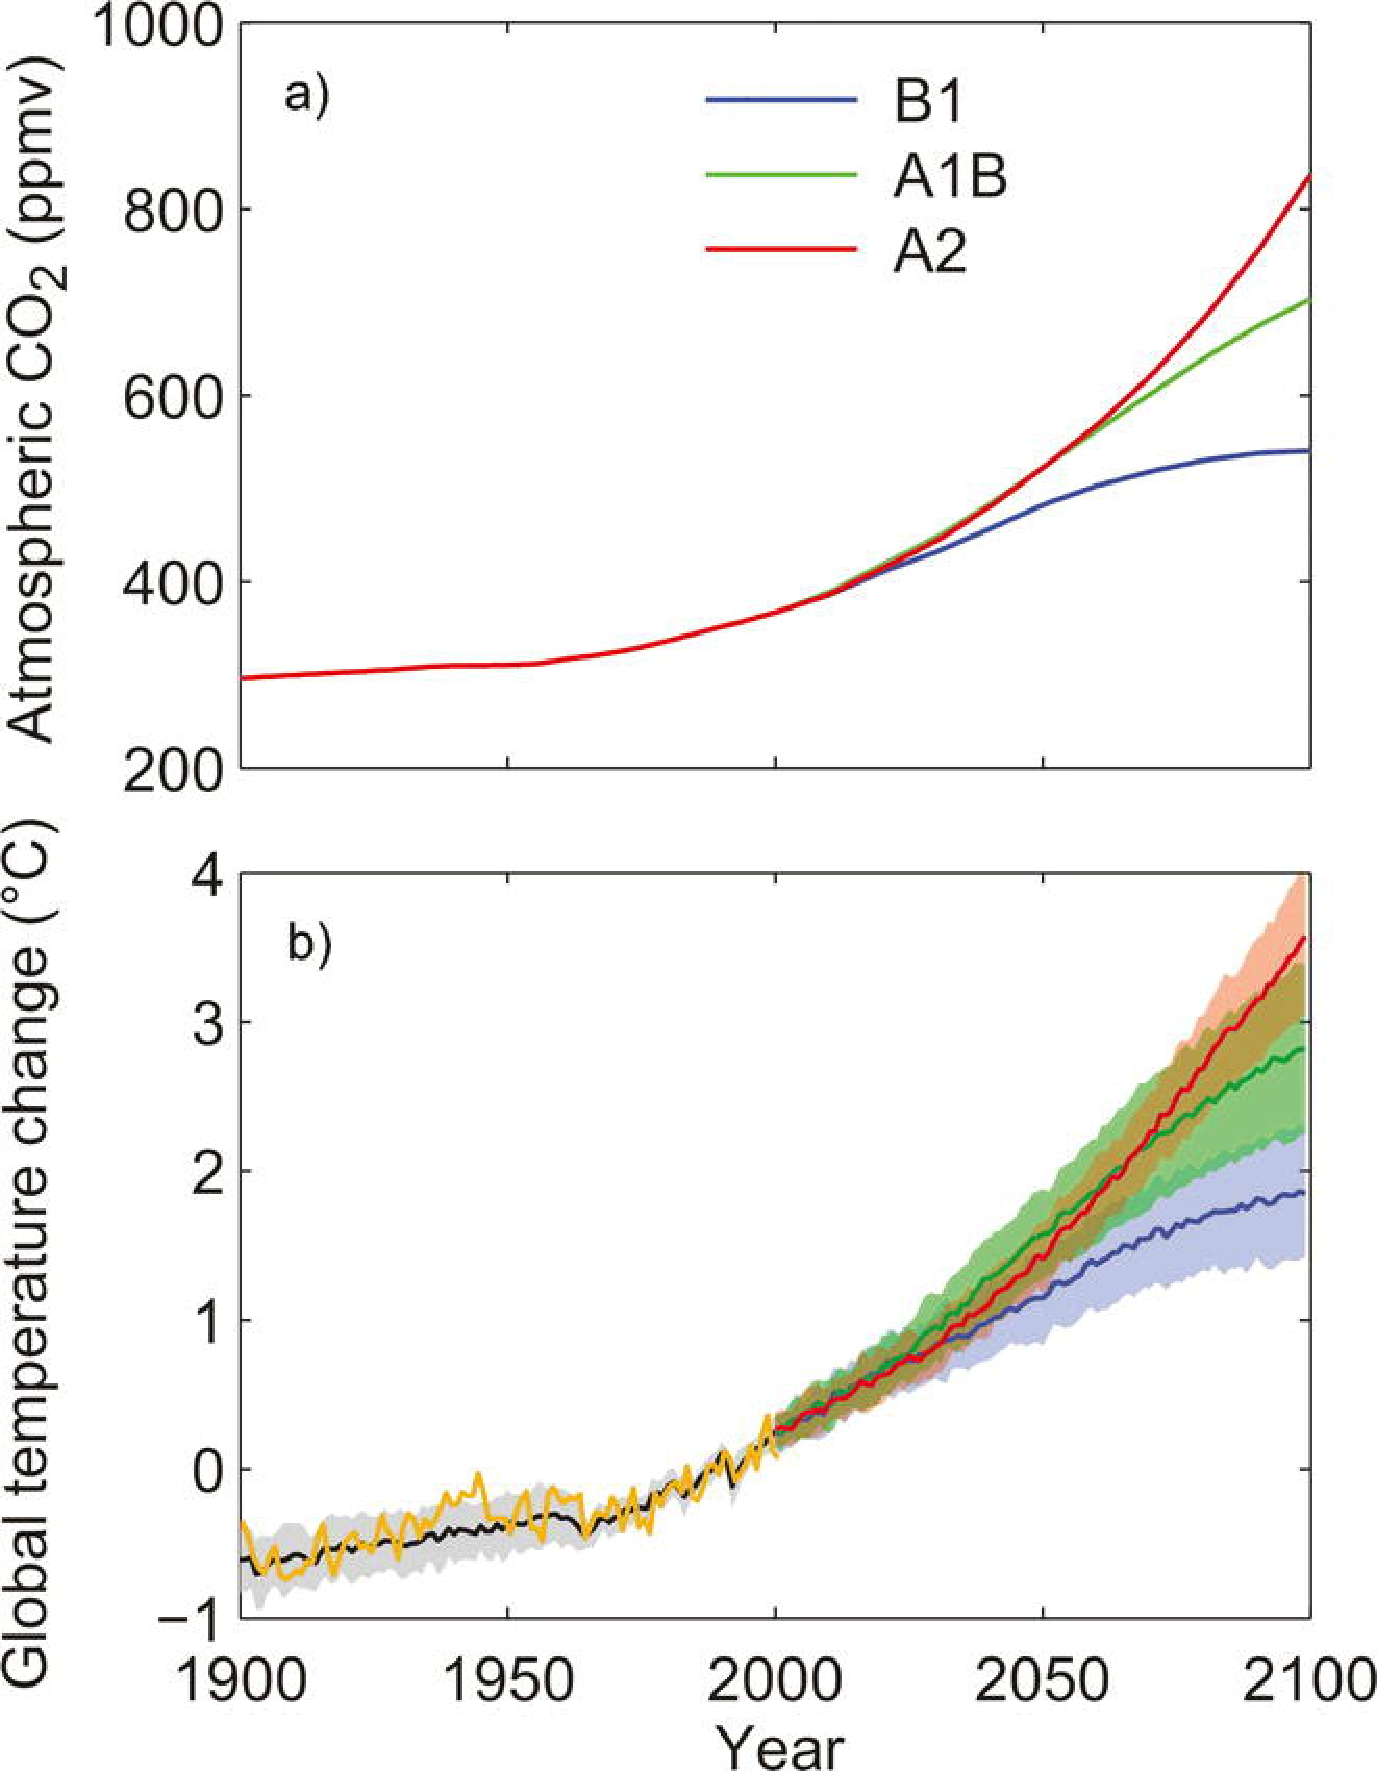
\includegraphics[width=19pc,angle=0]{figure01.pdf}\\
%  \caption{Enter the caption for your figure here.  Repeat as
%  necessary for each of your figures. Figure from \protect\cite{Knutti2008}.}\label{f1}
%\end{figure}

% NOTE: what to include in the paper, key questions.
% The paper should provide insight about what might happen if a large volcano erupted
% (order of magnitude or more than Mt.\ Pinatubo). How does the atmosphere react, for
% example in the aerosol dynamics? (QBO, SO2/AOD/RF relationship.) It should also be
% about how volcanic simulations compare in magnitude and if there is time for more
% simulations, how model complexity (dynamic ocean against slab ocean) affect things.
% - How far does the linear relation between AOD and RF go? What phases does the
%   aerosols go though? (Perhaps the most promising avenue.)
% - How much does it matter how high in the atmosphere the initial SO2 is injected?
%   (Already is some literature on this, suggesting it is not much. Also some on
%   latitude dependence, which has a bigger influence.)
% - How does the climate response change based on the state of the climate: what if we
%   run a CO2 doubling or quadrupling simulation until close to equilibrium, and let the
%   volcanoes erupt then? (Lack the doubling scenario, and setting it up has resulted in
%   strange output that must be resolved. Could take a while.)

\section{Introduction}

% NOTE: Suggested layout for the introduction
% - The objectives of the work.
% - The justification for these objectives: Why is the work important?
% - Background: Who else has done what? How? What have we done previously?
% - Guidance to the reader: What should the reader watch for in the paper? What are the
%   interesting high points? What strategy did we use?
% - Summary/conclusion: What should the reader expect as conclusion? In advanced
%   versions of the outline, you should also include all the sections that will go in
%   the Experimental section (at the level of paragraph subheadings) and indicate what
%   information will go.

% Toohey et al 2011 have a nice end of introduction.

\Gls{rf} and \gls{aod} are crucial metrics representing the energy imbalance at
\gls{toa} and the stratospheric opacity due to aerosol scattering, respectively. They
are extensively used to quantify the impact of major volcanic eruptions. The assumption
of a linear dependency of \gls{rf} on \gls{aod} is commonly adopted
\citep{myhre2013,andersson2015}, and applying such a linear relationship have yielded
reasonably accurate estimates in climate model simulations of volcanic eruptions
\citep{mills2017,hansen2005,gregory2016,marshall2020,pitari2016b}. Yet, there is a wide
spread in the estimated aerosol forcing efficiencies (\gls{rf} normalised by \gls{aod})
among studies, spanning approximately from \(\sim
\SI{15}{\watt\metre^{-2}\ce{AOD}^{-1}}\) \citep{pitari2016b} to \(\sim
\SI{25}{\watt\metre^{-2}\ce{AOD}^{-1}}\) \citep{myhre2013}. Additionally, these
estimates are predominantly based on small volcanoes with \gls{aod} values up to at most
\(\sim 0.7\).

Although \ce{H2O}, \ce{N2} and \ce{CO2} are the most abundant gases emitted by volcanoes
\citep{robock2000}, sulphur species such as \ce{SO2} provide greater influence due to
the comparatively high background concentrations of the former gases in the atmosphere.
The transformation of \ce{SO2} molecules through reactions with \ce{OH} and \ce{H2O}
leads to the formation of sulphate acid (\ce{H2SO4}) \citep{robock2000}, which scatter
sunlight hereby elevating planetary albedo and reducing the \gls{rf}. As the conversion
from \ce{SO2} to \ce{H2SO4} occurs over weeks \citep{robock2000}, the peak \gls{rf}
experiences a slight delay from the eruption's peak \ce{SO2} injection. The lifetime of
the \ce{H2SO4} aerosols in the stratosphere depends on various factors, including
latitude \citep{marshall2019, toohey2019}, volcanic plume height \citep{marshall2019},
aerosol size \citep{marshall2019}, the quasi-biennial oscillation phase
\citep{pitari2016b} and the season of the year (determining to which hemisphere aerosols
are transported) \citep{toohey2011,toohey2019}. In the case of tropical eruptions,
aerosols are typically transported poleward in the stratosphere and descend back to
mid-latitude troposphere within one to two years \citep{robock2000}. Upon descending
below the tropopause, these aerosols are readily removed by wet deposition
\citep{liu2012}.

Before the current era of significant anthropogenic climate forcing, volcanic eruptions
were the primary forcing mechanism dictating Earth's climate variability during the
Holocene period \citep{sigl2022}. Despite this substantial impact, few climate-model
experiments have included volcanic forcing when simulating climate evolution during the
Holocene \citep{sigl2022}, likely implying an exaggerated positive forcing
\citep{gregory2016,solomon2011}. This absence of persistent cooling is one of several
factors that have been suggested to contribute to the common disparity between simulated
and observed global warming \citep{andersson2015}. Despite extensive attention on
understanding the way volcanic eruptions influence climate, questions regarding aerosol
particle processes --- such as growth and creation rates when \ce{OH} is scarce ---
remain unanswered \citep[e.g.,][]{robock2000,zanchettin2019,marshall2020,marshall2022}.
These processes impact aerosol scattering efficiency and potentially the \gls{rf} to
\gls{aod} relationship. \citet{marshall2020} observed higher aerosol forcing efficiency
in post-eruption years \(2\) and \(3\) compared to year 1, and attributing this
post-eruption increase in aerosol forcing efficiency to strong spatial concentration in
the initial year and subsequent distribution of aerosols over a larger area. This
spatial redistribution increases the albedo per global mean \gls{aod} hereby causing a
stronger \gls{rf} to \gls{aod} ratio \citep{marshall2020}.

Previous studies of both Mt.\ Pinatubo \citep{mills2017,hansen2005} and volcanoes within
the instrumental era \citep{gregory2016} have been used to estimate the relationship
between the \gls{rf} energy imbalance and change in \gls{aod} caused by volcanic
eruptions. While \citet{myhre2013} employ a formula scaling \gls{rf} by \gls{aod} to
obtain \(\SI{-25}{\watt\metre^{-2}\mathrm{AOD}^{-1}}\), recent literature reports
estimates down to \(\SI{-19.0(5)}{\watt\metre^{-2}\mathrm{AOD}^{-1}}\)
\citep{gregory2016} and \(\SI{-18.3(10)}{\watt\metre^{-2}\mathrm{AOD}^{-1}}\)
\citep{mills2017}. Synthetic volcano simulations in \citet{marshall2020} yield a scaling
factor of \(\SI{-20.5(2)}{\watt\metre^{-2}\mathrm{AOD}^{-1}}\) across an ensemble of
\(82\) simulations featuring varying injection heights and latitudes of volcanic
emissions, with \iso{} ranging from \(10\) to \(\SI{100}{\tera\gram(\ce{SO2})}\).

A similar simulation setup, albeit with notable differences, was conducted by
\citet{niemeier2015}, involving an ensemble of \(14\) levels of injected sulphur
spanning between \(\SI{1}{\tera\gram(\ce{S})\mathrm{yr}^{-1}}\)
(\(\SI{2}{\tera\gram(\ce{SO2})\mathrm{yr}^{-1}}\)) and
\(\SI{100}{\tera\gram(\ce{S})\mathrm{yr}^{-1}}\)
(\(\SI{200}{\tera\gram(\ce{SO2})\mathrm{yr}^{-1}}\)). These geoengineering simulations
maintained continuous sulphur injections, running until a steady sulphur level was
achieved. Results indicated an inverse exponential relationship between \gls{rf} and
\iso{} rate, converging to \(\SI{-65}{\watt\metre^{-2}}\)
(Eq.~\ref{eq:niemeier_exponential}). Even the \(100\times\) Mt.\ Pinatubo super-volcano
simulation by \citet{jones2005}, which obtained a peak \gls{rf} of
\(\SI{-60}{\watt\metre^{-2}}\), is below the suggested limit of
\(\SI{-65}{\watt\metre^{-2}}\). Moreover, \citet{timmreck2010} find a peak \gls{rf}
anomaly of \(\SI{-18}{\watt\metre^{-2}}\) from a \(\SI{1700}{\tera\gram(\ce{SO2})}\)
eruption simulation, which corresponds well with the function estimated by
\citet{niemeier2015} at the given \ce{SO2} level.

One avenue that has garnered considerable attention is comparing the magnitude of
volcanic or volcano-like forcings to increased \ce{CO2} levels. Several studies explore
the connection between volcanic forcing and the climate sensitivity to a doubling of
\ce{CO2}
\citep{boer2007,marvel2016,merlis2014,ollila2016,richardson2019,salvi2022,wigley2005}.
This comparison aims to mitigate the large uncertainty in estimates of the sensitivity
of the real climate system. Inferring climate sensitivity from volcanic events has been
attempted as a way to constrain the sensitivity \citep{boer2007}, assuming that volcanic
and \ce{CO2} forcings produce similar feedbacks \citep{pauling2023}. Earlier studies
suggest the potential for constraining \gls{ecs} using volcanoes \citep{bender2010},
provided that \gls{ecs} is constrained by \gls{erf} rather than \gls{irf}, as \gls{erf}
accounts for rapid atmospheric adjustments in contrast to \gls{irf}
\citep{richardson2019}. However, other studies refute this approach, pointing out that
different sensitivities of volcanic forcing and \ce{CO2} doubling seem to exist
\citep{douglass2006}, or that constraining the \gls{ecs} by \gls{erf} lacks accuracy due
to the precision of climate simulations \citep{boer2007,salvi2022}. Although \gls{erf}
offers a more suitable indicator of forcing than \gls{irf}
\citep{marvel2016,richardson2019}, more recent studies conclude that \gls{ecs} cannot be
constrained from volcanic events \citep{pauling2023}.

Several studies have demonstrated a linear relationship of approximately
\(-\SI{20}{\watt\metre^{-2}\mathrm{AOD}^{-1}}\) between \gls{rf} and \gls{aod}, although
substantial variability exists in the slope among studies
\citep{mills2017,hansen2005,gregory2016,marshall2020,pitari2016b}. Moreover, a
time-after-eruption dependence on the \gls{rf} to \gls{aod} ratio is found in
\citet{marshall2020}, whereas \citet{niemeier2015} revealed a non-linear relationship
between \gls{rf} and \iso{} rate. Thus, a consensus on the relationship between \iso{},
\gls{aod} and \gls{rf} has yet to be established.

To address these issues, we conducted ensemble simulations of volcanic eruptions in the
\gls{cesm2} coupled with the \gls{waccm}. The ensembles span \iso{} levels of three
orders of magnitude with four members for each: \(\SI{26}{\tera\gram(\ce{SO2})}\),
\(\SI{400}{\tera\gram(\ce{SO2})}\) and \(\SI{1629}{\tera\gram(\ce{SO2})}\). Details
regarding the experimental setup are provided in section~\ref{sec:method}. Our findings
reveal clear non-linear \gls{rf} to \gls{aod} dependencies for medium to super-volcano
size eruptions. Additionally, we observe a time-dependent variation in the \gls{rf} to
\gls{aod} ratio, detailed in section~\ref{sec:results} and discussed in
section~\ref{sec:discussion}. Furthermore, our data, along with insights from previous
studies, suggest that the \gls{rf} dependency on \iso{} identified by
\citet{niemeier2015} acts as a lower boundary. Our conclusions are presented in
section~\ref{sec:conclusions}.

\section{Method}\label{sec:method}

\subsection{Model}

We utilised the \gls{cesm2} \citep{danabasoglu2020} in conjunction with the \gls{waccm}
\citep{gettleman2019} and the fully dynamical ocean component \gls{pop}
\citep{smith2010, danabasoglu2020}. The atmosphere model was run at nominal
\(\SI{2}{\degree}\) resolution with \(70\) vertical levels in the \gls{ma}
configuration.

The \gls{waccm} version employed in the \gls{ma} configuration uses the \gls{mam3}
\citep{gettleman2019}, a simplified and computationally efficient default setting within
the \gls{cam5} \citep{liu2016}, as described in \citet{liu2012}. The \gls{mam3} was
developed from MAM7, consisting of the seven modes Aitken, accumulation, primary carbon,
fine dust, fine sea salt, coarse dust and coarse sea salt. Instantaneous internal mixing
of primary carbonaceous aerosols with secondary aerosols and instantaneous ageing of
primary carbonaceous particles is assumed by emitting primary carbon in the accumulation
mode \citep{liu2016}. As dust absorbs water efficiently and is expected to be removed by
wet deposition similarly to sea salt, fine dust is merged with fine sea salt into the
accumulation mode and coarse dust is merged with coarse sea salt into a coarse mode.
% Fine sea salt is assimilated into the accumulation mode, and as dust absorbs water
% efficiently, aerosols are expected to be removed by wet deposition similarly to sea
% salt, allowing fine dust to be merged into the accumulation mode as well. Likewise,
% coarse dust is merged with coarse sea salt into a coarse mode, and as both absorb
% water efficiently, 
The coarse mode will quickly retain its background state below the tropopause
\citep{liu2012}. Consequently, \gls{mam3} features the three modes Aitken, accumulation
and coarse \citep{liu2016}.

\subsection{Simulations}

Appendix A provides a detailed description of the simulation setup and utilised output
variables. Table~\ref{tab:simulation-overview} summarizes the simulations, encompassing
three \ce{SO2} injection magnitudes across four seasons: February 15th, May 15th, August
15th, and November 15th. The magnitudes vary over three orders of magnitude:
\(\SI{26}{\tera\gram(\ce{SO2})}\), \(\SI{400}{\tera\gram(\ce{SO2})}\), and
\(\SI{1629}{\tera\gram(\ce{SO2})}\).

The smallest eruption case, \gls{c2wm}, is similar in magnitude as compared to events
like Mt.\ Pinatubo
\citep[\(\sim10\)--\(\SI{20}{\tera\gram(\ce{SO2})}\);][]{timmreck2018} and Mt.\ Tambora
\citep[\(\sim\SI{56.2}{\tera\gram(\ce{SO2})}\);][]{zanchettin2016}. The intermediate
case, \gls{c2wmp}, resembles the Samalas eruption in 1257
\citep[\(\sim{118.8}\)--\(\SI{173.1}{\tera\gram(\ce{SO2})}\);][]{toohey2017,ottobliesner2016},
while the largest eruption case, \gls{c2ws}, is similar to the \gls{ytt} eruption
occurring about \(\SI{75000}{\mathrm{yr}}\) ago
\citep[\(100\)--\(\SI{10000}{\tera\gram(\ce{SO2})}\);][]{jones2005}. All eruptions were
situated at the equator (\(\SI{0}{\degree N}\), \(\SI{1}{\degree E}\)) with \ce{SO2}
injected between \(\SI{18}{\kilo\meter}\) and \(\SI{20}{\kilo\meter}\) altitude.
Collectively, the three eruption cases \gls{c2wm}, \gls{c2wmp} and \gls{c2ws} are
referred to as \gls{c2w}. Two additional high-latitude eruptions, labelled \gls{c2wsn},
of the same \iso{} magnitude as \gls{c2ws} were simulated at \(\SI{56}{\degree N}\),
\(\SI{287.7}{\degree E}\) with a six-month separation (February 15th and August 15th).

Employing eruptions in the medium to super-volcano size enhances the signal-to-noise
ratio without necessitating an extensive and computationally expensive ensemble, and as
such, is a tempting way to mimic a large ensemble of smaller volcanic eruptions.
However, there is no guarantee that the \gls{aod}, \gls{rf} and temperature signatures
will be a simple scaling of that of smaller volcanic eruptions. Previous studies have
simulated super-volcanoes using \gls{aod} as the input forcing, where the \gls{aod} was
that of Mt.\ Pinatubo scaled by one hundred \citep{jones2005}. This approach may yield
incorrect results, both since the peak of the \gls{aod} may be too small or big, but
also since the evolution of the \gls{aod} could be wrong. Similarly, a different
\gls{aod} evolution may be found from similar size volcanoes, but at different
latitudes. To avoid this issue, we \dots

\begin{table*}
  \centering

  \caption{\gls{cesm2} simulations. The ensembles \gls{c2wsn} and \gls{c2ws} have the same
    eruption magnitude, but while \gls{c2ws} is located at the equator, \gls{c2wsn} is
    located at high northern latitude. \gls{c2wmp} and \gls{c2wm} are located at the
    equator, but with different magnitudes as compared to \gls{c2ws}. All tropical ensembles
    have four members, indicated by the amount of eruption months, while the northern
    latitude ensemble consist of two members}\label{tab:simulation-overview}%
  \begin{center}
    \begin{tabular}[c]{cccc}
      Ensemble name                                                                    & \(\si{\tera\gram(\ce{SO2})}\)         &
      Lat, lon, alt [\si{\degree\mathrm{N}}, \si{\degree\mathrm{E}}, \si{\kilo\metre}] & Eruption months                         \\
      \gls{c2wsn}                                                                      & \(1629\)                              &
      \(56\), \(287.7\),
      \(18\)--\(20\)                                                                   & Feb,\hphantom{May,}Aug\hphantom{,Nov}   \\
      \gls{c2ws}                                                                       & \(1629\)                              &
      \(\hphantom{1}0\), \(\hphantom{28}1\hphantom{.7}\), \(18\)--\(20\)
                                                                                       & Feb,May,Aug,Nov                         \\
      \gls{c2wmp}                                                                      & \(\hphantom{1}400\)                   &
      \(\hphantom{1}0\),
      \(\hphantom{28}1\hphantom{.7}\),
      \(18\)--\(20\)                                                                   & Feb,May,Aug,Nov                         \\
      \gls{c2wm}                                                                       & \(\hphantom{14}26\)                   &
      \(\hphantom{1}0\),
      \(\hphantom{28}1\hphantom{.7}\), \(18\)--\(20\)
                                                                                       & Feb,May,Aug,Nov                         \\
    \end{tabular}
  \end{center}
\end{table*}

\section{Results}\label{sec:results}

% NOTE: the results should be laid out in a logical way, with the most
% interesting/important stuff first, then tangents that dig deeper at specific things
% later.
% 1. RF to AOD time-after-eruption dependence should be top priority (8 figs atm.)
% 2. Then probably temperature scaling since we discuss the shape of both AOD and RF
%    time series before that (MOTIVATION: can we expect a specific temperature time
%    series shape based on the shape of either of or both of the RF and AOD time
%    series?)
% 3. If there is something interesting to say about the rest of the figures (all the
%    comparing of parameters), then this should come here.

\subsection{Analysis of the time series}

Figure~\ref{fig:compare-waveform-temp} illustrates time series of global mean \gls{aod},
\gls{rf}, and surface air temperature. The black lines represent the medians across the
four-member ensembles, while shading indicates the 5th to 95th percentiles. The three
distinct forcing magnitudes (\gls{c2wm}, \gls{c2wmp}, and \gls{c2ws}) outlined in
table~\ref{tab:simulation-overview} have been used. The time series in
Fig.~\ref{fig:compare-waveform-temp} are normalised by setting the peak value to unity,
defined based on the peak of a fit from a Savitzky-Golay filter of 3rd order and a
one-year window length \citep{savitzky1964}.

A notable feature across all three subfigures of Fig.~\ref{fig:compare-waveform-temp} is
the earlier peak occurrence of the \gls{c2wm} case compared to the larger eruption
cases. Cases \gls{c2wmp} and \gls{c2ws} peak at similar times, but \gls{c2wmp} exhibits
a faster rise and slower decay in the \gls{aod} time series
(Fig.~\ref{fig:compare-waveform-temp}a). Generally, the \gls{aod} time series from
stronger eruption cases seem to display a sharper peak, or a slower rise and faster
decay. The rise in RF across the three eruption cases in
Fig.~\ref{fig:compare-waveform-temp}b is similar, although \gls{c2wm} reaches the peak
just prior to the other two cases. During the decay phase, all cases appear to decay at
a similar rate, however maintaining the offset caused by the earlier peak arrival of
\gls{c2wm}. Cases \gls{c2wmp} and \gls{c2ws} exhibit indistinguishable \gls{rf} time
series. Similarly, when observing the temperature evolution in
Fig.~\ref{fig:compare-waveform-temp}c, \gls{c2wmp} and \gls{c2ws} are indistinguishable,
while \gls{c2wm} has a sharper peak relative to the two other cases. Nevertheless,
across all cases for the parameters shown in Fig.~\ref{fig:compare-waveform-temp}, a
similar temporal development is found. Therefore, similar dynamics are expected to be at
play in all cases.

\begin{figure}
  \centering
  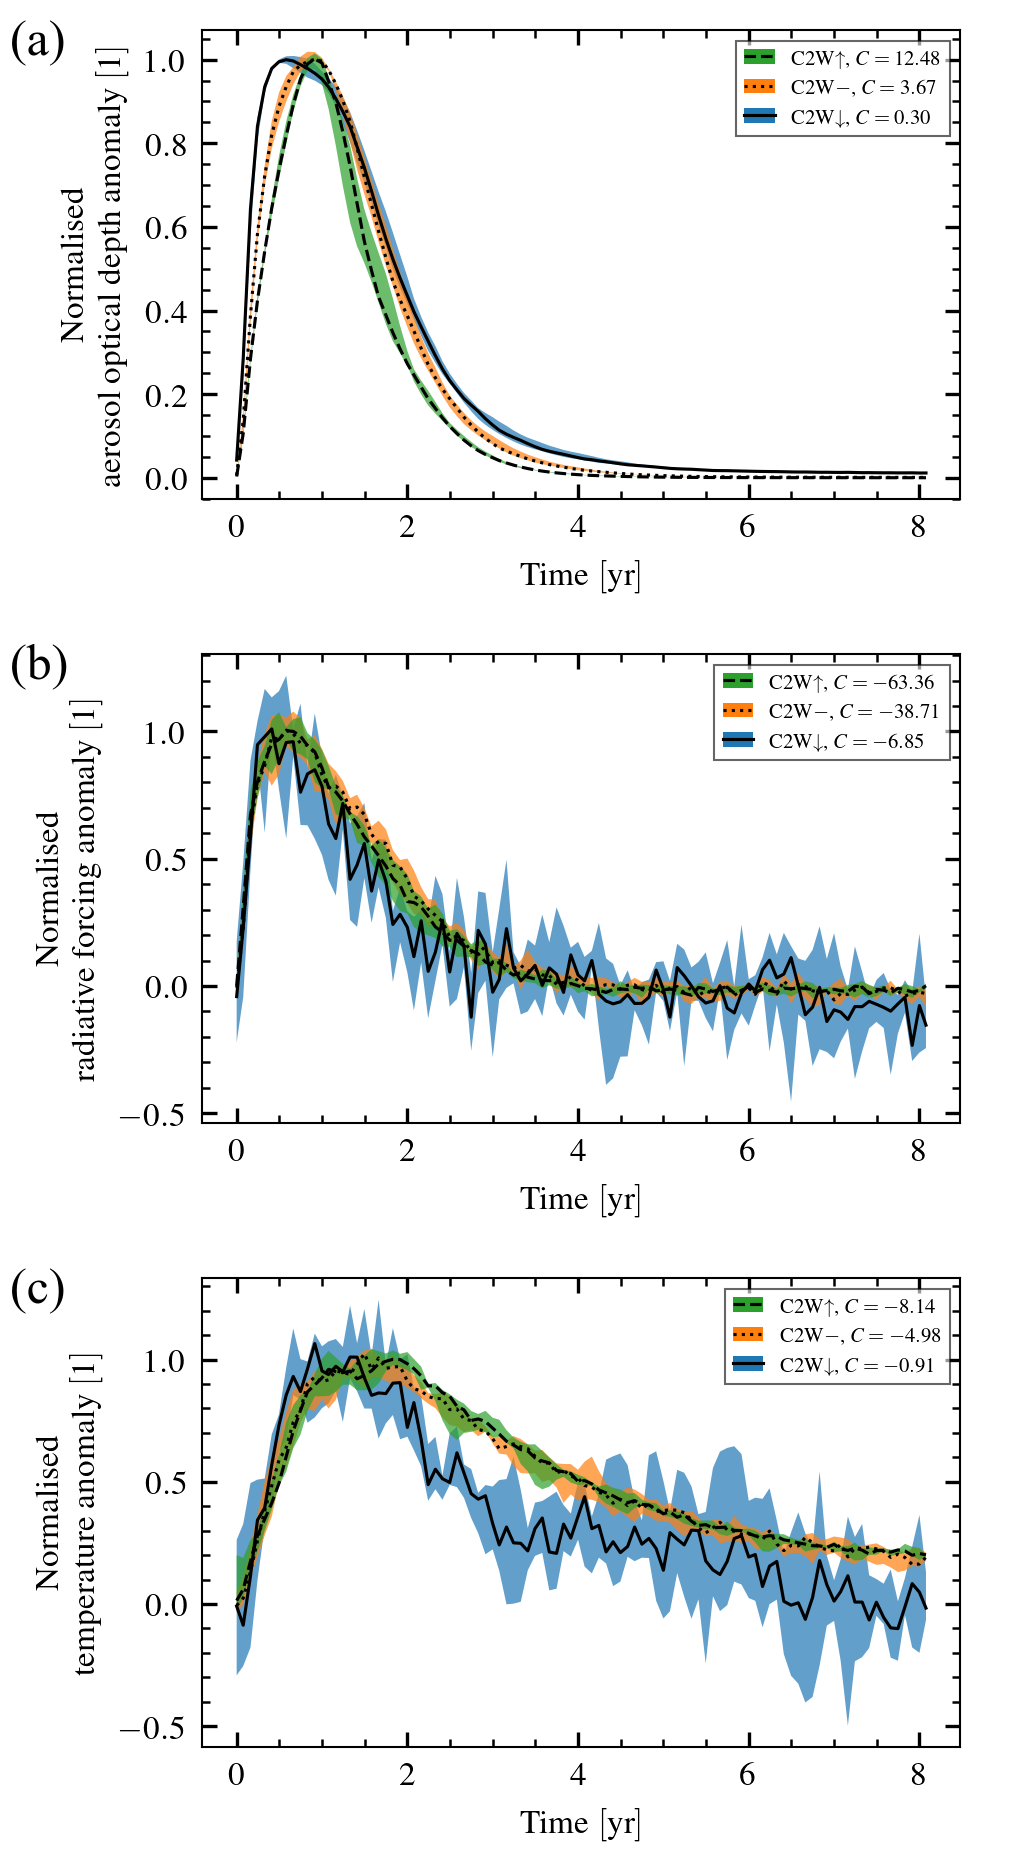
\includegraphics{figures/figure1.png}

  \caption{\gls{aod} (a), \gls{rf} (b) and temperature response (c) time series to the
    three tropical volcanic eruption cases, \gls{c2wm}, \gls{c2wmp} and \gls{c2ws}. The time
    series have been normalised to have peak values at unity, where \(C\) is the
    normalisation constant. Black lines indicate the median across the four-member
    ensembles, while shading marks the 5th and 95th
    percentiles.}\label{fig:compare-waveform-temp}%
\end{figure}

Upon asking whether the shape of the temperature time series can be inferred from the
shape of either of the forcing time series (\gls{aod} or \gls{rf}), we find that the
shapes of the \gls{rf} time series are consistent over the different eruption strengths
(Fig.~\ref{fig:compare-waveform-temp}b), suggesting a strong dependence of temperature
on \gls{rf}. About the same can largely be said about the \gls{aod} time series, though
they show a slight change in shape from smaller to larger eruptions
(Fig.~\ref{fig:compare-waveform-temp}a). Specifically, the \gls{aod} time series from
smaller eruptions displays a fast rise and a flat peak before decaying back to its
equilibrium state. From the larger eruptions, we find a slower rise but a sharper peak,
resulting in a decay to equilibrium happening at a similar time after the eruption and
at a similar rate.

\subsection{\gls{rf} dependency on \gls{aod}}

We next focus on the development of the \gls{aod} and \gls{rf} time series relative to
each other. Similar comparisons were conducted in \citet[][their Fig.\ 4]{gregory2016}
and \citet[][their Fig.\ 1]{marshall2020}, with \gls{rf} plotted against \gls{aod}.
Figure~\ref{fig:aod_vs_toa_ses_avg} displays annual mean values from the four simulation
cases in table~\ref{tab:simulation-overview}; the small eruption case (\gls{c2wm}) as
blue downward pointing triangles, the intermediate eruption case (\gls{c2wmp}) as orange
thick diamonds, the large tropical eruption case (\gls{c2ws}) as green upward pointing
triangles, and the large northern hemisphere eruption case (\gls{c2wsn}) as brown upward
pointing three-branched twigs. Also shown are the data from \citet[][Fig.\ 4, black
  crosses from HadCM3 sstPiHistVol]{gregory2016} as grey crosses labelled \gls{g16}
(described in Appendix B, section~\ref{ap:g16}). Additionally, the estimated peak values
from the Mt.\ Pinatubo and Mt.\ Tambora eruptions are plotted as a black star and plus,
while the peak from the \citet{jones2005} simulation is shown as a pink square labelled
\gls{j05}. Finally, red circles represent the peak values obtained from the \gls{c2w}
tropical eruption cases. The straight lines are the same as shown by
\citet{gregory2016}. The full data range is shown in Fig.~\ref{fig:aod_vs_toa_ses_avg}a
while Fig.~\ref{fig:aod_vs_toa_ses_avg}b highlights a narrow range, focusing on the
\gls{c2wm} case.

The annual mean data from the Pinatubo-like \gls{c2wm} case in
Fig.~\ref{fig:aod_vs_toa_ses_avg}b have \gls{rf} values as a function of \gls{aod} that
follow almost the same constant slope as the \gls{g16} data. However, in
Fig.~\ref{fig:aod_vs_toa_ses_avg}a we observe that the stronger eruptions lead to
dissimilar responses in \gls{aod} and \gls{rf}, where \gls{c2wmp} seems to follow close
to a \(-10\) slope and \gls{c2ws} is closer to a \(-5\) slope. The peak values (red
circles) suggest a non-linear dependence, while within each eruption strength (same
colour) the annual mean values fall relatively close to a straight line.

\begin{figure}
  \centering
  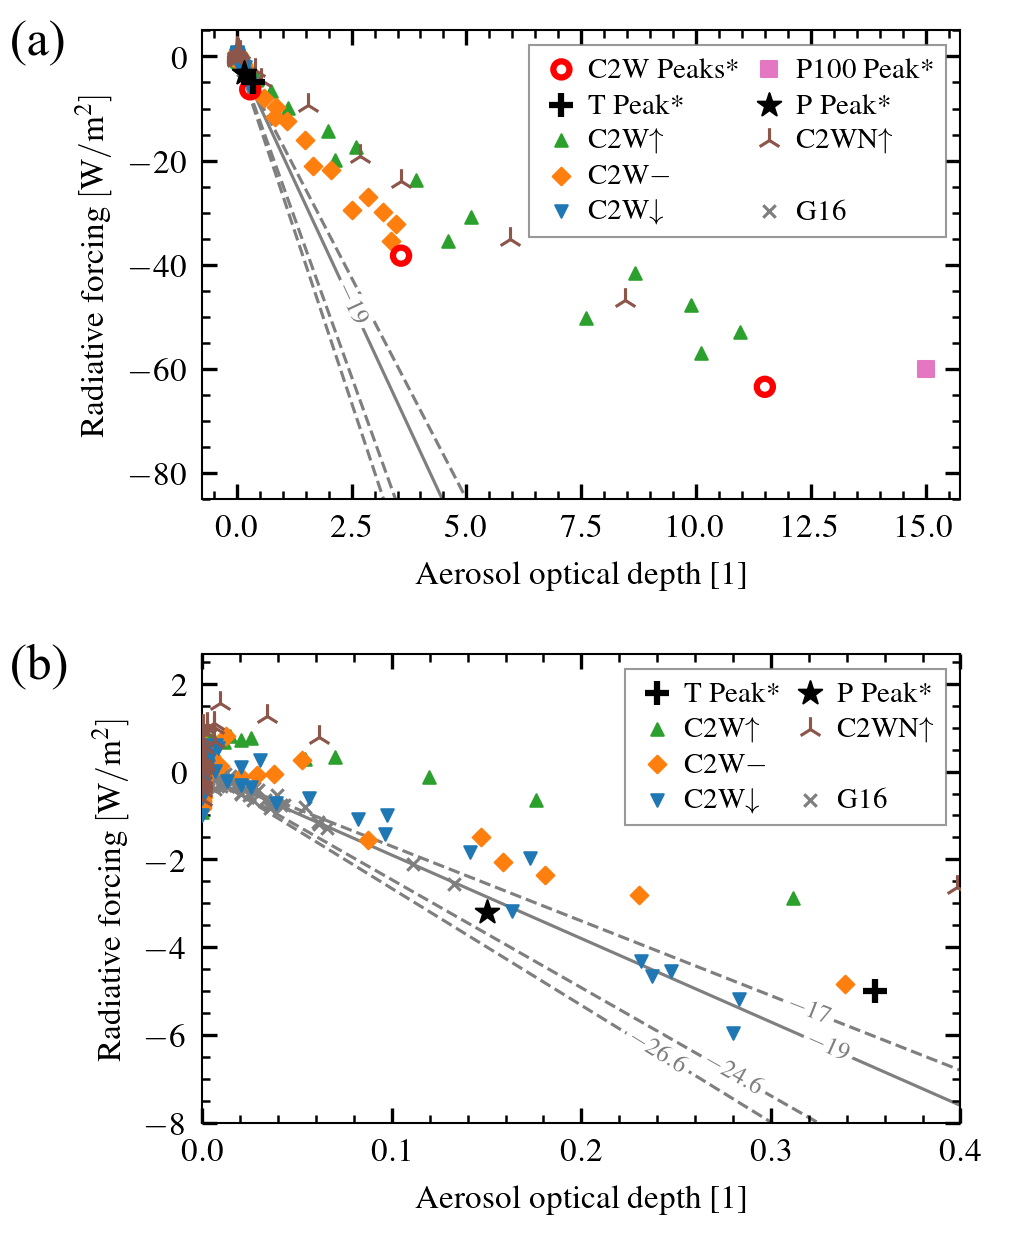
\includegraphics{figures/figure2.png}

  \caption{\gls{rf} as a function of \gls{aod}, yearly means. Data from the four
    simulations listed in table~\ref{tab:simulation-overview} (\gls{c2wm}, \gls{c2wmp},
    \gls{c2ws} and \gls{c2wsn}) are shown along with the data from the HadCM3 sstPiHistVol
    simulation by \citet{gregory2016} (grey crosses, \gls{g16}). Also shown are the
    estimated peak values of the Mt.\ Pinatubo (black star) and Mt.\ Tambora (black plus)
    eruptions. In (a) the simulated super-volcano of \citet{jones2005} (pink square) is
    shown, as well as the peak values from the simulations \gls{c2wm}, \gls{c2wmp} and
    \gls{c2ws} (red circles). All peak values (as opposed to annual means) have an asterisk
    (\(\ast{}\)) in their label. The grey lines are the same regression fits as in
    \citet[][Fig.\ 4]{gregory2016}, where the solid line is the fit to \gls{g16}. (b):
    Zooming in on the smallest \gls{aod} values.}\label{fig:aod_vs_toa_ses_avg}%
\end{figure}

To find the development of \gls{aod} and \gls{rf} relative to each other over time, we
plot in Fig.~\ref{fig:aod_vs_toa_avg_loop_ratios} seasonal means of the \gls{rf} to
\gls{aod} ratio, where the start of the time series is taken as the eruption day. The
plot shows all the eruption cases given in table~\ref{tab:simulation-overview}, as well
as the tropical eruptions from the \citet{marshall2020dataset} dataset (\(6\) of \(82\)
eruptions), labelled \gls{m20} and described in Appendix B, section~\ref{ap:m20}. In
Fig.~\ref{fig:aod_vs_toa_avg_loop_ratios}a, slopes are linear regression fits to the
seasonal means across all ensemble members, summarised in
table~\ref{tab:slope-gradients}. Shaded regions are the standard deviation around the
seasonal means. A similar shading is plotted in
Fig.~\ref{fig:aod_vs_toa_avg_loop_ratios}b, but where the regression fits have been
omitted for clarity. Years \(1\) and \(2\) have the lowest signal-to-noise ratio, as
well as year \(0\) (the noise is mostly due to the \gls{rf} time series, shown in
Fig.~\ref{fig:compare-waveform-temp}b). For this reason, the ratio of \gls{rf} to
\gls{aod} is calculated for the second season of the first year until the end of the
third year.

Although the ratio changes across the eruption magnitudes, we find that all the tropical
cases (\gls{c2w}) follow a positive slope during the first period, as seen in
Fig.~\ref{fig:aod_vs_toa_avg_loop_ratios}a and described in
table~\ref{tab:slope-gradients}. A positive slope is also found from the tropical
eruptions in the \gls{m20} dataset. The northern latitude case in \gls{c2wsn} show a
much flatter slope compared to \gls{c2w} and \gls{m20}. The distinction between the
slopes from the tropical and non-tropical cases is perhaps more clear in
Fig.~\ref{fig:aod_vs_toa_avg_loop_ratios}b and corresponding rows in
table~\ref{tab:slope-gradients}. Again, \gls{c2wsn} show an almost flat slope compared
to the tropical cases. During the second period more noise is introduced, but a weak
tendency of negative slopes is found among the tropical cases.

\begin{table}
  \centering

  \caption{Slope and standard deviation for the data in
    Fig.~\ref{fig:aod_vs_toa_avg_loop_ratios}. The regression fits in the top half of the
    table are for Fig.~\ref{fig:aod_vs_toa_avg_loop_ratios}a, while the bottom half is for
    Fig.~\ref{fig:aod_vs_toa_avg_loop_ratios}b. The columns ``1st period'' and ``2nd
    period'' refer to the period year \(0\)--\(1\) and \(1\)--\(3\), respectively. The
    ensembles are the same as those given in table~\ref{tab:simulation-overview}, in
    addition to the \(6\) tropical eruptions from the \(82\) member ensemble in
    \citet{marshall2020}.}\label{tab:slope-gradients}%
  \begin{tabular}{cccc}
    Figure                                                  & Ensemble name & 1st period      & 2nd period       \\
    \rowcolor{LightGray}                                    & \gls{c2wsn}   & \(0.45\pm1.15\) & \(1.51\pm1.45\)  \\
    \rowcolor{LightGray}                                    & \gls{c2ws}    & \(3.85\pm0.52\) & \(-3.29\pm0.60\) \\
    \rowcolor{LightGray}                                    & \gls{c2wmp}   & \(4.36\pm0.82\) & \(-3.37\pm0.59\) \\
    \rowcolor{LightGray}                                    & \gls{c2wm}    & \(3.64\pm2.41\) & \(-1.41\pm3.25\) \\
    \rowcolor{LightGray}                                    & \gls{m20}     & \(6.34\pm1.77\) & \(-0.36\pm1.33\) \\
    \multirow{5}{*}{\ref{fig:aod_vs_toa_avg_loop_ratios}b}  & \gls{c2wsn}   & \(0.08\pm0.20\) & \(0.27\pm0.26\)  \\
    \multirow{-9}{*}{\ref{fig:aod_vs_toa_avg_loop_ratios}a} & \gls{c2ws}    & \(0.75\pm0.10\) & \(-0.64\pm0.12\) \\
                                                            & \gls{c2wmp}   & \(0.43\pm0.08\) & \(-0.34\pm0.06\) \\
                                                            & \gls{c2wm}    & \(0.18\pm0.12\) & \(-0.07\pm0.16\) \\
                                                            & \gls{m20}     & \(0.33\pm0.07\) & \(-0.02\pm0.08\) \\
  \end{tabular}
\end{table}

\citet[][their Fig.\ 1c,d]{marshall2020} present results that demonstrate a
time-dependent relationship in the conversion between \gls{aod} and \gls{rf}. Contrary
to the results from the \gls{c2w} cases, they obtain an \gls{rf} to \gls{aod} ratio with
a negative slope over time. As such, \citet{marshall2020} find that the aerosol forcing
efficiency increases with time rather than decrease. This phenomenon is explained by
\citet{marshall2020} as the aerosols initially are spatially confined to the hemisphere
where the eruption occurred. Subsequently, during the second and third years, they
spread globally, resulting in a higher global-mean albedo per \gls{aod} and consequently
stronger \gls{rf} per \gls{aod} ratio with time. However, this included the full
\(82\)-member ensemble. When constraining the ensemble to only include eruptions within
\(-10\) to \(\SI{10}{\degree\mathrm{N}}\), we obtain the positive slope as stated above
and shown in Fig.~\ref{fig:aod_vs_toa_avg_loop_ratios} and
table~\ref{tab:slope-gradients}. Therefore, the much flatter slope of \gls{c2wsn} should
be expected based on the results from \citet{marshall2020}, which indicate that tropical
eruptions contribute to a positive slope while high-latitude eruptions contribute to a
negative slope. As a result, the aerosol forcing efficiency seems strongly dependent on
eruption latitude.

\begin{figure}
  \centering
  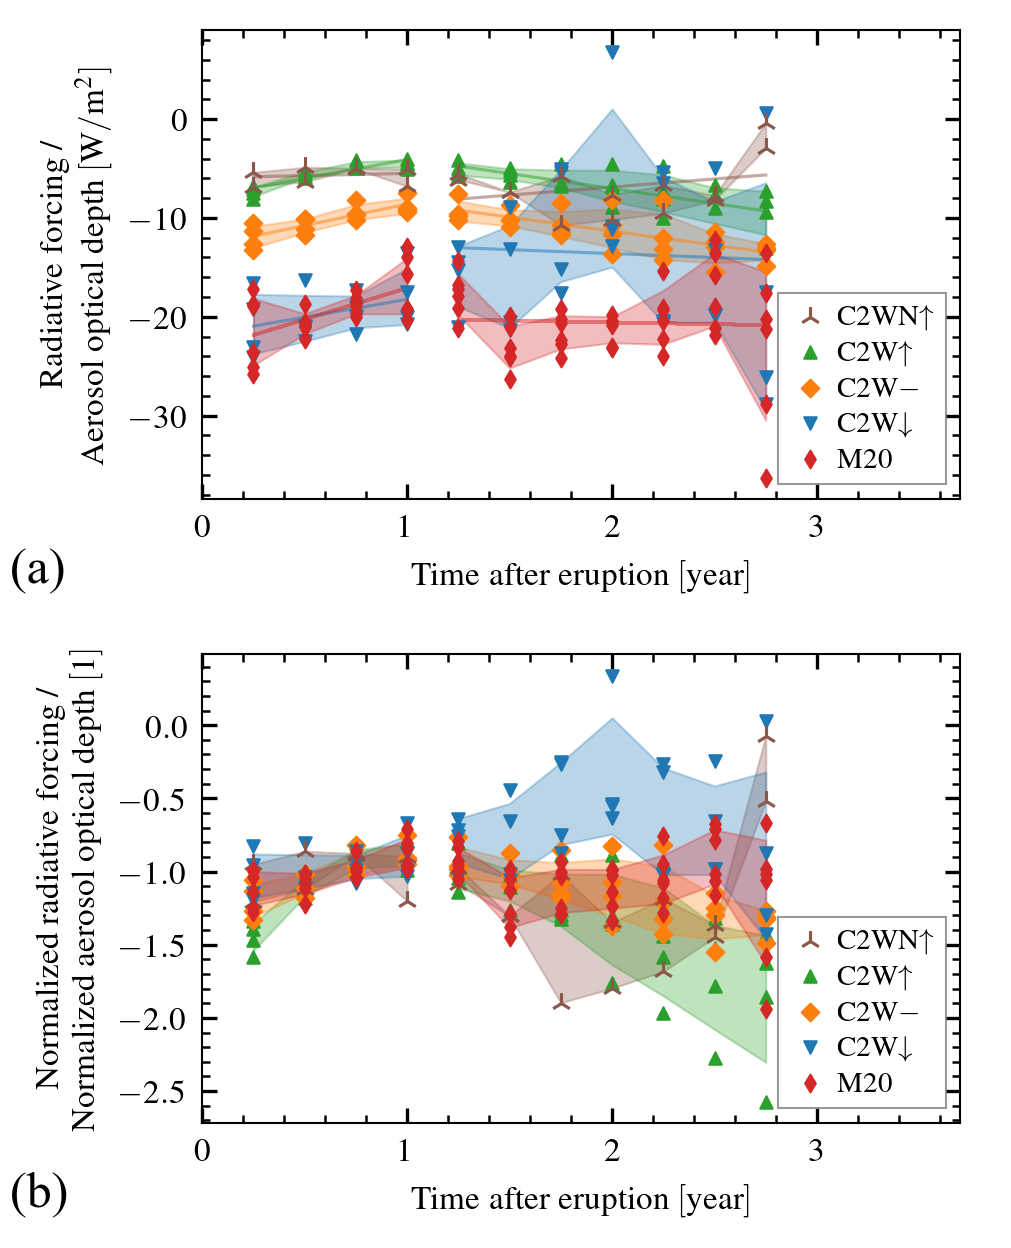
\includegraphics{figures/figure3.png}

  \caption{(a): The ratio of \gls{rf} to \gls{aod}, with time-after-eruption on the
    horizontal axis. Straight lines indicate linear regression fits and are described in
    table~\ref{tab:slope-gradients}, while shaded regions are the standard deviation across
    the ensembles for each season. (b): Same as in (a), but where the underlying \gls{aod}
    and \gls{rf} time series have been scaled to have peak values at unity. Shown are data
    from table~\ref{tab:simulation-overview} along with tropical eruptions from
    \gls{m20}.}\label{fig:aod_vs_toa_avg_loop_ratios}%
\end{figure}

\subsection{Parameter scan}

In Fig.~\ref{fig:parameter_scan}, we compare all relevant parameters against each other.
The primary input parameter in the \gls{cesm2} is \iso{}. For our tropical cases
(\gls{c2w}), we observe an almost linear relationship between \gls{aod} peak values
against \iso{}. The latitude also plays a role for the magnitude of the \gls{aod}
perturbation, evident from \gls{c2wsn}. This weak yet significant latitude dependence
aligns with findings by \citet{marshall2019}, indicating that \(\SI{72}{\percent}\) of
the \gls{aod} variance can be attributed to \iso{}, while latitude accounts for only
\(\SI{16}{\percent}\) of the variance. Peak values from their data (82 simulations)
plotted as red thin diamonds displays a similar pattern, with \gls{aod} exhibiting close
to linear dependence on \iso{}, but with latitude introducing a spread in \gls{aod}.
Peak values from Mt.\ Pinatubo (P) and Mt.\ Tambora (T) are shown for reference, along
with peak values from \citet{jones2005} labelled \gls{j05} and \citet{timmreck2010}
labelled \gls{t10}.

The almost linear relationship between \gls{aod} and \iso{} for the \gls{c2w} data
suggest a comparable trend for \gls{rf} versus \iso{} as seen in \gls{rf} versus
\gls{aod}. This relationship along with the functional relationships between all other
parameters shown in Fig.~\ref{fig:parameter_scan} are illustrated in
Fig.~\ref{fig:diagram_function_relations}. There, we find that by assuming a linear
dependency of \gls{aod} on \iso{} (\(ax+b\)), and of temperature on \gls{rf} (\(cx+d\)),
we must have that \(f\), \(g\), \(h\) and \(k\) all have the same functional form, where
\(f: \ce{SO2} \to \mathrm{RF}\), \(g: \mathrm{AOD} \to \mathrm{T}\), \(h: \ce{SO2} \to
\mathrm{T}\) and \(k: \mathrm{AOD} \to \mathrm{RF}\). From this, we deduce that
\(f(x)=k(ax+b)\) and \(h(x)=f(cx+d)=g(ax+b)\), and finally that \(h(x)=k(acx+ad+b)\)
with the conclusion that \(f\), \(g\), \(h\) and \(k\) have the same functional form.

In Fig.~\ref{fig:parameter_scan}b, \gls{rf} plotted against \iso{} (with the
absolute value of \gls{rf} on the \(y\)-axis) indicates a substantial damping effect on
\gls{rf} as \iso{} increases for the \gls{c2w} data, in agreement with results from
\citet{ottobliesner2016}, labelled \gls{ob16}. The analysis details of \gls{ob16} can be
found in Appendix B, section~\ref{ap:ob16}. Despite the model complexity difference,
\citet{ottobliesner2016}'s simulations using \gls{cesm1} with a low-top atmosphere
(\gls{cam5}) produce \glspl{rf} comparable to our findings.

\begin{figure*}
  \centering
  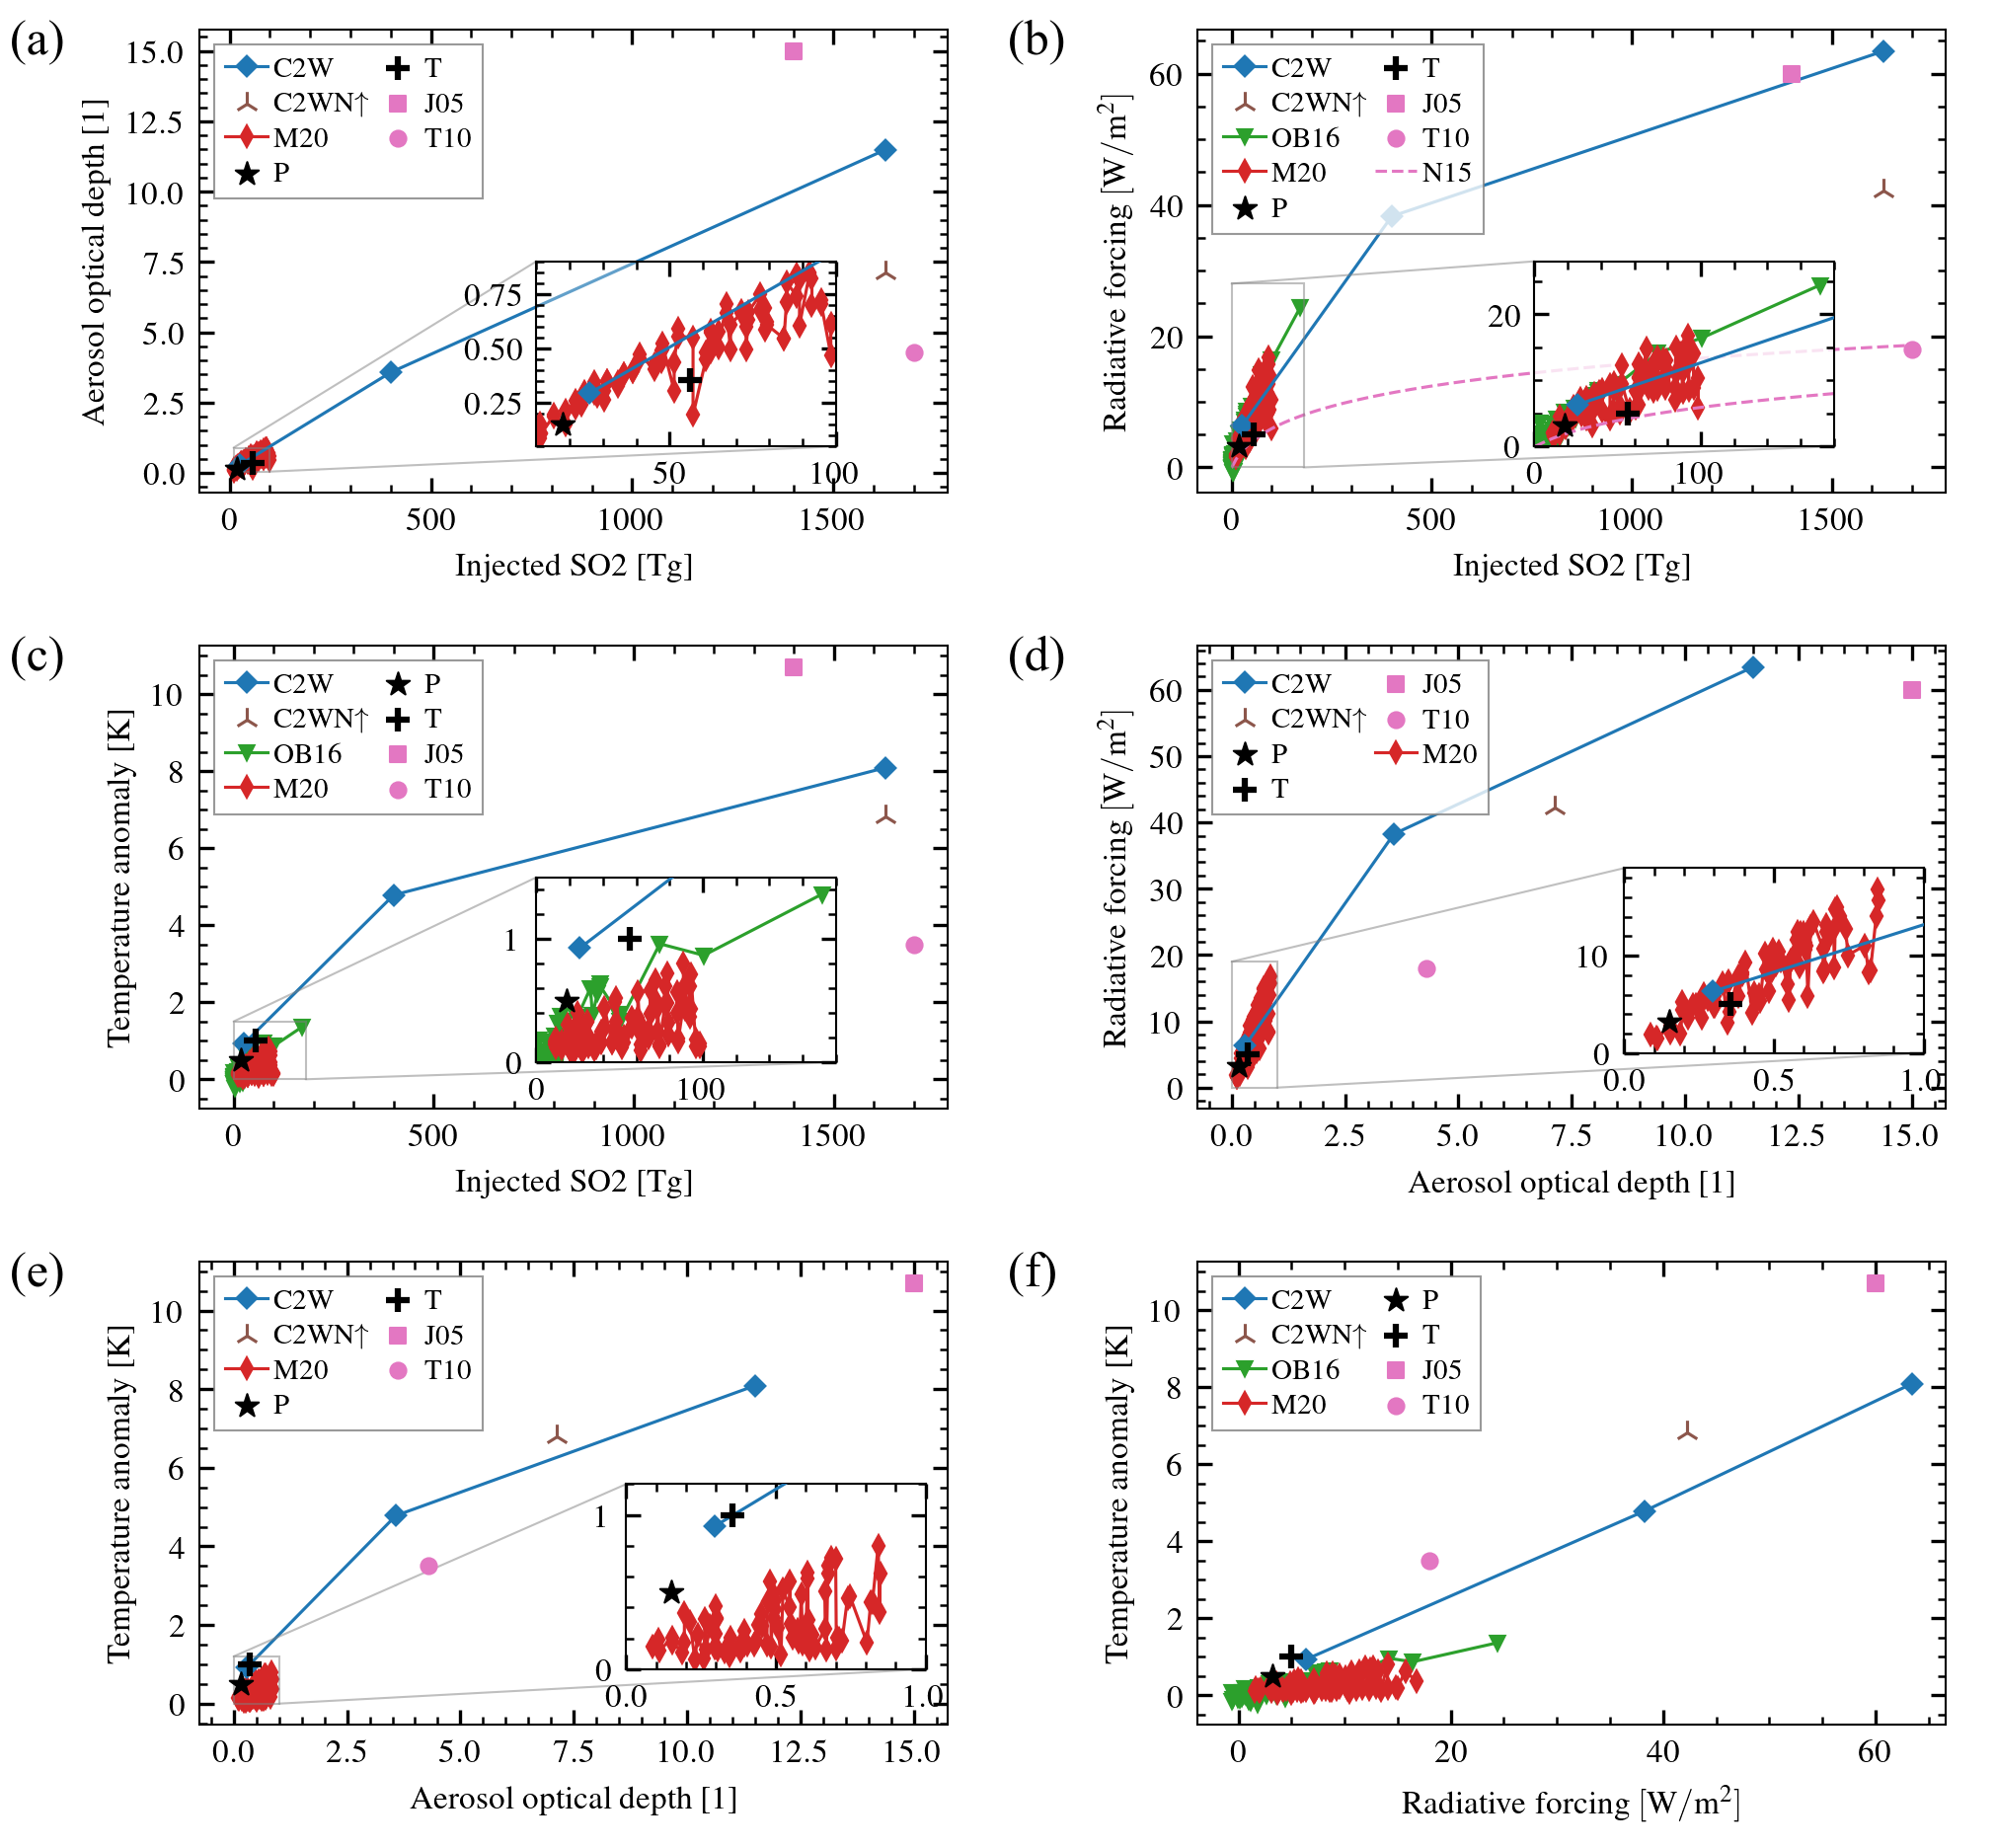
\includegraphics{figures/figure4.png}

  \caption{(a) \gls{aod} (b) \gls{rf} and (c) temperature anomaly as a function of
    \iso{}\@. (d) \gls{rf} and (e) temperature anomaly as a function of \gls{aod}. (f)
    Temperature anomaly as a function of \gls{rf}. Blue diamonds labelled \gls{c2w}
    represent tropical cases (\gls{c2wm}, \gls{c2wmp}, \gls{c2ws}), the brown three-branched
    twig signifies the \gls{c2wsn} case, and green downward triangles denote \gls{ob16} data
    from \citet{ottobliesner2016}. The red thin diamonds labelled \gls{m20} display the
    \citet{marshall2020dataset} data. Black star and plus indicate Mt.\ Pinatubo and Mt.\
    Tambora estimates based on observations. The pink square labelled \gls{j05} refers to
    the one-hundred times Mt.\ Pinatubo super-volcano from \citet{jones2005}, and the pink
    disk labelled \gls{t10} represents the \gls{ytt} super-volcano from
    \citet{timmreck2010}. The pink dashed line labelled \gls{n15} is from
    \citet{niemeier2015}, indicating the function in
    Eq.~\ref{eq:niemeier_exponential}.}\label{fig:parameter_scan}%
\end{figure*}

\begin{figure}
  \centering

  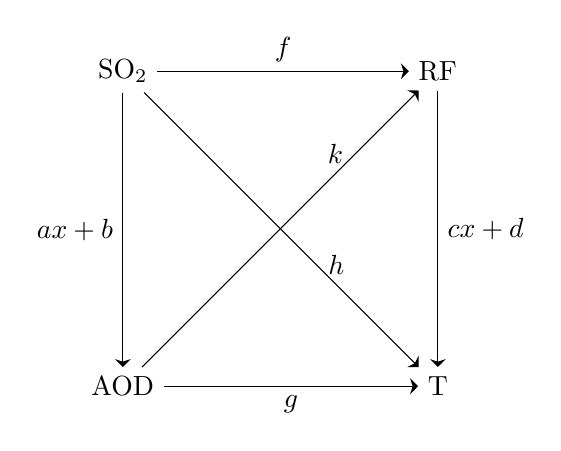
\begin{tikzpicture}[>={Stealth[length=1mm,width=2mm]}]
    % Place the letters in the corners
    \node (A) at (0,0) {AOD}; \node (T) at (4,0) {T}; \node (RF) at (4,4) {RF}; \node (S) at
    (0,4) {\ce{SO2}};
    % Draw arrows between the letters
    \draw[->] (A) -- node[midway, below] {\(g\)} (T); \draw[->] (RF) -- node[midway, right]
    {\(cx+d\)} (T); \draw[->] (S) -- node[midway, above] {\(f\)} (RF); \draw[->] (S) --
    node[midway, left] {\(ax+b\)} (A); \draw[->] (S) -- node[pos=0.7, above] {\(h\)} (T);
    \draw[->] (A) -- node[pos=0.7, above] {\(k\)} (RF);
  \end{tikzpicture}

  \caption{Diagram describing the functional relationships of the parameters shown in
  Fig.~\ref{fig:parameter_scan}.}\label{fig:diagram_function_relations}%
\end{figure}

% INFO: the conversion between S and SO2 is confirmed by Niemeier and Timmreck (2015)'s
% reference to the Bekki et al. (1996) paper. Bekki uses 6000 Mt SO2, Niemeier uses 3000
% Tg(S).
\citet{niemeier2015} conducted simulations of continuous sulphur injections up to
\(\SI{200}{\tera\gram(\ce{SO2})\mathrm{yr}^{-1}}\) in the ECHAM5's middle atmosphere
version \citep{giorgetta2006} with aerosol microphysics from HAM \citep{stier2005}. They
observed an \gls{rf} dependence on \ce{SO2} injection rate following an inverse
exponential, which converges to \(\SI{-65}{\watt\meter^{-2}}\), depicted in
Fig.~\ref{fig:parameter_scan}b as the stippled pink line labelled \gls{n15} and given
as;

\begin{equation}
  \Delta
  R_{\mathrm{TOA}} =
  -\SI{65}{\watt\metre^{-2}}
  \mathrm{e}^{-{\left(\frac{\SI{2246}{\tera\gram(S)yr^{-1}}}{x}\right)}^{0.23}}.
  \label{eq:niemeier_exponential}
\end{equation}
%
Both our simulations and \gls{ob16} exhibit a notably faster increase than this
exponential relationship. However, \gls{t10} closely correspond to the function in
Eq.~\ref{eq:niemeier_exponential}. Starting from an initial input of
\(\SI{850}{\tera\gram(\ce{S})}\) (equivalent to \(\SI{1700}{\tera\gram(\ce{SO2})}\),
representing the \gls{ytt} eruption), their estimated \gls{aod} led to a peak \gls{rf}
of \(\SI{-18}{\watt\metre^{-2}}\) (pink filled circle in
Fig.~\ref{fig:parameter_scan}b). These results were from a simulation utilising the
MPI-ESM climate model, driven by \gls{aod} data from the HAM aerosol model. Thus, the
alignment likely stem from using the same aerosol microphysical model in
\citet{timmreck2010} and \citet{niemeier2015}, alongside applying highly similar climate
models, MPI-ESM and ECHAM5, respectively \citep{kuma2023}. The climate model family
relations are further examined in Appendix C. Notably, the peak values from \gls{m20}
align well within an upper boundary defined by \gls{c2w} and \gls{ob16}, and a lower
boundary defined by Eq.~\ref{eq:niemeier_exponential}. Eruptions closer to the equator
within \gls{m20} correspond to data points near the upper boundary, while eruptions at
more extreme latitudes yield weaker peak \gls{rf} values being closer to the lower
boundary. Crucially, none of the eruption simulations violated the suggested upper
threshold of \(\SI{-65}{\watt\metre^{-2}}\) as defined in
Eq.~\ref{eq:niemeier_exponential}.

Figure~\ref{fig:parameter_scan}c illustrates the response of temperature against \iso{}.
Similar to Fig.~\ref{fig:parameter_scan}b, the increase of temperature response with
\iso{} decreases for higher \iso{}. Notably, \gls{ob16} takes a different trajectory
compared to \gls{c2w}, showing smaller temperature dependence on \iso{}. In contrast to
our findings, \gls{t10} finds a considerably weaker temperature perturbation, noting a
maximum temperature anomaly of only \(\SI{-3.5}{\kelvin}\) for their
\(\SI{1700}{\tera\gram(\ce{SO2})}\) eruption, while \gls{j05} records a substantially
larger maximum temperature anomaly of \(\SI{-10.7}{\kelvin}\) compared to our \gls{c2w}
simulations.

Moving to Fig.~\ref{fig:parameter_scan}d, we revisit the relationship between \gls{rf}
and \gls{aod}, focusing on peak values rather than annual and seasonal averages. As
previously discussed, the \gls{rf} to \gls{aod} ratio displays weaker slopes than
previous studies \citep{jones2005, marshall2020, timmreck2010}, with the \gls{c2w} peak
values not conforming to a linear trend. This comparison suggests potential significant
dependencies on the model and its input parameters, such as latitude, but most notably
to an inherent non-linear \gls{rf} dependence on \gls{aod}. Both the \gls{g16} and
\gls{j05} data originate from the same climate model, and similarly to what we find from
the \gls{c2w} data, the ratio is much stronger for small eruptions in the industrial era
(\gls{g16}) compared to the super-volcano eruption (\gls{j05}).

For Fig.~\ref{fig:parameter_scan}e, \gls{c2w} should resemble the patterns observed in
Fig.~\ref{fig:parameter_scan}c due to the nearly linear association identified between
\gls{aod} and \iso{} in Fig.~\ref{fig:parameter_scan}a. This is indeed the case, and in
addition both the \gls{c2wsn} and the \gls{j05} cases align well, with the \gls{t10}
case following a similar dependence. \gls{m20} shows temperature anomalies of smaller
extent, similar to what was found in Fig.~\ref{fig:parameter_scan}c. However, the
\gls{m20} experiment was conducted with prescribed sea-surface temperatures
\citep{marshall2020}, preventing the temperature from being fully perturbed.

Finally, in Fig.~\ref{fig:parameter_scan}f, we compare the temperature and \gls{rf}
responses. Both \gls{c2w} and \gls{ob16} show a near-linear relationship between
temperature and \gls{rf}. The \gls{c2w} data indicate a steeper slope, potentially
implying stronger temperature perturbations compared to \gls{ob16}. However, there are
potential biases in the values from the analysis of the \gls{ob16}, as outlined in
Appendix B, section~\ref{ap:ob16}. This, along with considerable noise, result in the
analysis of \gls{ob16} being less reliable. As in Fig.~\ref{fig:parameter_scan}e, the
\gls{c2wsn} case along with the \gls{j05} and \gls{t10} cases closely follow the
temperature to \gls{rf} dependence of \gls{c2w}.

\section{Discussion}\label{sec:discussion}

% NOTE: Suggested layout for the
% Discussion:
% - Explain the results and emphasize significant findings clearly
% - Discuss the impact and importance of results compared with recent relevant research
% Conclusion
% - The justification for these objectives: Why is the work important?
% - Summarize the key points made in the other sections
% - Conclude overall discussion of article
% - Link this section to the introduction

\subsection{Linearity between \gls{aod} and \gls{rf}}

Figures~\ref{fig:aod_vs_toa_ses_avg},~\ref{fig:aod_vs_toa_avg_loop_ratios} and
\ref{fig:parameter_scan}d demonstrate that as the \gls{aod} exceeds approximately
\(1.0\), the linear \gls{rf} dependence of approximately
\(\SI{-20}{\watt\metre^{-2}\mathrm{AOD}^{-1}}\) no longer hold. The almost linear
relationship between \gls{aod} and \iso{} in Fig.~\ref{fig:parameter_scan}a indicates
that larger eruptions, injecting more \ce{SO2}, lead to larger aerosols, and hence less
effective radiation scattering, thereby reducing the \gls{rf} for the same \gls{aod}
\citep{english2013, timmreck2010, timmreck2018}.

\citet{timmreck2010} highlights that for sufficiently large eruptions such as Mt.\
Pinatubo and \gls{ytt}, \ce{OH} radicals are too scarce, which limit \ce{SO2} oxidation.
The \gls{aod} peak in the \gls{ytt} simulation of \citet{timmreck2010} occur six months
after Mt.\ Pinatubo's peak. This result aligns with our findings, as illustrated in
Fig.~\ref{fig:compare-waveform-temp}a, where smaller eruptions show an earlier \gls{aod}
peak. While \citet{timmreck2010} reports a peak \gls{rf} anomaly occurring \(7\)--\(8\)
months post-eruption, \citet{jones2005} suggests a peak anomaly one year post-eruption.
The \gls{rf} peak preceding the \gls{aod} peak, approximately \(6\)--\(8\) months
post-eruption in \gls{cesm2} (see Fig.~\ref{fig:compare-waveform-temp}b), aligns well
with what was found by \citet{timmreck2010} for the \gls{ytt}. Hence, both the \gls{aod}
and \gls{rf} time series appear influenced by the \iso{} magnitude and the \ce{OH}
abundance, affecting the peak timing as well as the magnitude.

Although \gls{j05} is comparable to \gls{c2ws} concerning \gls{aod} and \gls{rf} peak
values, the temperature response reported by \citet{jones2005} appears much stronger
than what our strongest eruption leads too. Since \citet{jones2005} multiplies the
\gls{aod} time series from Mt.\ Pinatubo by one hundred to represent the \gls{aod} time
series of a super-volcano, this simple approach could potentially deviate significantly
from the real \gls{aod} time series of the super-volcano, both in shape and magnitude.
In addition, it may cause a substantially different temperature perturbation.
\citet{timmreck2010} obtained their \gls{aod} estimate from an initial injection of
\ce{SO2}, which resulted in a delayed peak, but also much smaller peak compared to that
of \gls{j05}. Also, the maximum temperature perturbation of \gls{t10} is much smaller
than that of \gls{j05}, largely due to the large difference in \gls{aod} magnitude.
Since in addition the \gls{j05} temperature is greater than that from \gls{c2ws}, it is
expected that the shape of the \gls{aod} time series is also important in determining
the strength of the aerosol forcing and corresponding temperature perturbation.

The biggest spread in the data is found when converting from \iso{} to any of the three
output parameters when comparing across models. Conversion from \iso{} to \gls{aod} is
consistent within similar models, even when comparing simulations of volcanic eruptions
\citep{timmreck2010} and continuous injection of \ce{SO2} \citep{niemeier2015}, but has
a wide spread at large values of \iso{} across model families
(Figs.~\ref{fig:parameter_scan}a,b,c). Comparatively, the \gls{rf}
(Fig.~\ref{fig:parameter_scan}d) and temperature (Fig.~\ref{fig:parameter_scan}e) as a
function of \gls{aod} demonstrate a smaller spread across models, and consequently, the
spread for temperature as a function of \gls{rf} (Fig.~\ref{fig:parameter_scan}f) is
also small. Previous studies assumed a roughly linear relationship between \gls{rf} and
\gls{aod}, particularly for lower values of \gls{aod} and \gls{rf}, where the estimated
slope was notably steeper at around \(\SI{-20}{\watt\metre^{-2}\mathrm{AOD}^{-1}}\) for
\(\mathrm{AOD}<1\) compared to the approximately
\(\SI{-5}{\watt\metre^{-2}\mathrm{AOD}^{-1}}\) observed here at \(\mathrm{AOD}\gg1\).
Hence, a linear relationship appears to be an accurate estimate of \gls{rf} dependence
on \gls{aod} for eruptions similar to or smaller than Mt.\ Pinatubo. However, for larger
eruptions, factors like \ce{OH} scarcity and aerosol growth, influencing reflectance,
and their gravitational pull substantially impact both \gls{aod} and \gls{rf} evolution.

From the \gls{c2w} cases, a post-eruption time dependence on the \gls{rf} to \gls{aod}
ratio emerges. \citet{marshall2020} discusses a similar aspect, finding that aerosol
forcing efficiency strengths from year 1 to year 2. This is by \citet{marshall2020}
attributed to the time taken for aerosol dispersion, affecting global albedo and
consequently \gls{rf}, whereas \gls{aod} is less affected by aerosol dispersion. Here,
the aerosol forcing efficiency become weaker during the first period, as depicted in
Fig.~\ref{fig:aod_vs_toa_avg_loop_ratios}. Focusing solely on tropical eruptions in
\gls{m20} (between \(-10\) and \(\SI{10}{\degree\mathrm{N}}\)), the \gls{rf} to
\gls{aod} ratio closely resembles the findings from the \gls{c2wm} case. Thus, while
\iso{} is crucial for estimating the time-average of the \gls{rf} to \gls{aod} ratio,
latitude and in particular aerosol dispersion seem more influential in determining the
post-eruption evolution of the ratio. Given that the \gls{c2wsn} case lack a significant
increase in ratio as compared to \gls{c2w}, the substantial difference in eruption
latitude appears to be a likely cause.

\citet{marshall2019, marshall2020, marshall2021} utilise a code with seven log-normal
modes to simulate aerosol mass and number concentrations, along with an atmosphere-only
configuration of the UM-UKCA with prescribed sea-surface temperatures and sea-ice extent
\citep{marshall2019}. This approach is in contrast with \gls{cesm2}, operating as an
\gls{esm}, but with a simpler aerosol chemistry model in the \gls{mam3}. The family of
models to which \gls{m20} is based is different from that of \gls{c2w}, and also
different from the \gls{t10} and \gls{n15}, as described in Appendix C. Based on
Fig.~\ref{fig:parameter_scan}, the model family seems pivotal in determining the
estimated \gls{aod} and \gls{rf} magnitudes from \iso{}, whereas the various models
generally demonstrate more consistency in representing \gls{rf} from \gls{aod}. Given
that \gls{m20} employs a model from a distinct family compared to both \gls{ob16} and
\gls{c2w}, and \gls{t10} and \gls{n15}, while covering the parameter space between the
two families, it would be intriguing to include higher \iso{} values in the \gls{m20}
experiments to explore whether \gls{rf} against \iso{} remains bounded below (by
\gls{t10} and \gls{n15}) and above (by \gls{ob16} and \gls{c2w}), as
Fig.~\ref{fig:parameter_scan}b indicate. This also prompts questions about whether
\ce{SO2} saturation at a specific level yields a lower bound on the corresponding peak
\gls{rf} response, and if this peak \gls{rf} response is similar to what a high-latitude
eruption would produce. Alternatively, differences in model aerosol chemistry may be
what produces the wide range in \gls{rf} as a function of \iso{}.

In summary, smaller eruptions and their impact produce a relatively well defined
\gls{rf} to \gls{aod} ratio (\(\sim \SI{-20}{\watt\metre^{-2}\mathrm{AOD}^{-1}}\)),
whereas larger eruptions result in estimates with smaller magnitudes (\(\sim
\SI{-10}{\watt\metre^{-2}\mathrm{AOD}^{-1}}\) to \(\sim
\SI{-5}{\watt\metre^{-2}\mathrm{AOD}^{-1}}\), as depicted in
Fig.~\ref{fig:aod_vs_toa_avg_loop_ratios}). \citet{niemeier2017} indicate a decrease in
aerosol forcing efficiency as the injection rate increases, due to larger volcanic
eruptions leading to larger aerosol particles that scatter sunlight less efficiently,
thereby decreasing the forcing efficiency per \iso{} \citep{english2013, timmreck2018}.

\subsection{Climate sensitivity estimate}

As previously mentioned, \gls{j05} agree well with \gls{c2ws} concerning both \gls{aod}
and \gls{rf} values, yet differ in temperature. To investigate this discrepancy, we here
conduct a comparison between their climate feedback parameter \(\alpha \) (where
\(s=1/\alpha \) is the climate sensitivity parameter) with our climate resistance,
denoted as \(\rho \), and the \gls{tcrp} \(1/\rho\) (where
\(\mathrm{TCS}=F_{2\times}\times \mathrm{TCRP}\) is the transient climate sensitivity).
As forcing of volcanic eruptions typically last for about a year, a duration too brief
for the timescales at which \(F=\rho T\) remains valid \citep{gregory2016}, an
alternative approach involves using a time-integral form introduced by
\citet{merlis2014}:

\begin{equation}
  \int_0^{\tau}F \mathrm{d}t=\rho\int_{0}^{\tau}T \mathrm{d}t
\end{equation}
\begin{equation}
  \rho=\frac{\int_0^{\tau}F \mathrm{d}t}{\int_{0}^{\tau}T \mathrm{d}t}.
  \label{eq:climate-resistance}
\end{equation}

If the upper bound of the integral, \(\tau \), is sufficiently large, so that the upper
ocean heat content is the same at \(t=0\) and \(t=\tau \), this approach agrees with
\(F=\rho T\) for long-term forcing \citep{gregory2016} (\citet{merlis2014} utilised
\(\tau =\SI{15}{\mathrm{yr}}\)). Additionally, it is worth noting that the climate
resistance and the climate feedback parameter are associated with the ocean heat uptake
efficiency (\(\kappa \)) through \(\rho =\alpha +\kappa \) \citep{gregory2016}.

The climate feedback parameter estimated by \citet{jones2005} is \(\alpha \simeq
\SI{4}{\watt\metre^{-2}\kelvin^{-1}}\), exceeding twice the value obtained by
\citet{gregory2016} in their simulations of Mt.\ Pinatubo using the same HadCM3 climate
model. We determine the climate resistance using the integral-form computation outlined
in Eq.~\ref{eq:climate-resistance} and adopting \(\tau =\SI{20}{\mathrm{yr}}\). The
estimated climate resistance from the three tropical simulation cases (with four in each
ensemble) yields \(\rho =\SI{3(2)}{\watt\metre^{-2}\kelvin^{-1}}\), and \gls{tcrp}
values of \(1/\rho=\SI{0.39(9)}{\kelvin\watt^{-1}\metre^{2}}\), as reported in
table~\ref{tab:trcp}. One outlier was found in the dataset from the \gls{c2wm} case, and
omitting this ensemble member results in \(\rho
=\SI{2.4(2)}{\watt\metre^{-2}\kelvin^{-1}}\) and \(1/\rho
=\SI{0.41(4)}{\kelvin\watt^{-1}\metre^{2}}\).

Even after \(20\) years, the temperature has not fully recovered, as seen in
Fig.~\ref{fig:compare-waveform-temp}. Yet, we assume the estimate of \(\rho
=\SI{2.4(2)}{\watt\metre^{-2}\kelvin^{-1}}\) to be a good estimate of \(\alpha \).
Importantly, the estimate of \(\alpha \simeq \SI{4}{\watt\metre^{-2}\kelvin^{-1}}\) by
\citet{jones2005} is still significantly larger than our estimate, similar to what
\citet{gregory2016} found.

Since the temperature perturbation obtained by \gls{j05} was higher than achieved here,
it indicates that the forcing used by \gls{j05} must be stronger. Even though the
\gls{aod} peak value used by \gls{j05} was \(100\) times that of Mt.\ Pinatubo, the
\gls{rf} peak value was only about \(20\) times that of Mt.\ Pinatubo
\citep{gregory2016}. From the results shown here, this reduced aerosol forcing
efficiency for large volcanic eruptions is expected and akin to the \gls{rf} dependency
on \gls{aod} found here. By inspection of Fig.~\ref{fig:parameter_scan} we find that the
aerosol forcing efficiency is somewhat smaller in \gls{j05}. We therefore expect the
primary contributor to the overall increased forcing strength to originate from the
development of the forcing time series, not the magnitude.

\begin{table}
  \centering

  \caption{Estimated climate resistance and \gls{tcrp} by use of the method outlined by
    \citet{merlis2014}. Estimates are based on ensembles with four members and \(\tau
    =\SI{20}{\mathrm{yr}}\) using Eq.~\ref{eq:climate-resistance}. One ensemble member
    within \gls{c2wm} had an outlier, and the same estimate but with this outlier removed is
    indicated as ``w/o outlier'' (without outlier).}\label{tab:trcp}%
  \begin{tabular}{ccc}
    Simulation type          & \(\rho [\si{\watt\metre^{-2}\kelvin^{-1}}]\) & \(1/\rho\)        \\
    \gls{c2ws}               & \(\num{2.2(1)}\)                             & \(\num{0.45(2)}\) \\
    \gls{c2wmp}              & \(\num{2.5(1)}\)                             & \(\num{0.39(2)}\) \\
    \gls{c2wm}               & \(\num{4(3)}\)                               & \(\num{0.3(1)}\)  \\
    \gls{c2wm} (w/o outlier) & \(\num{2.5(3)}\)                             & \(\num{0.40(4)}\) \\
    Total                    & \(\num{3(2)}\)                               & \(\num{0.39(9)}\) \\
    Total (w/o outlier)      & \(\num{2.4(2)}\)                             & \(\num{0.41(4)}\) \\
  \end{tabular}
\end{table}

% C2W^:         2.2+-0.1        0.45+-0.02
% C2W-:         2.5+-0.1        0.39+-0.02
% C2W_:         4+-3            0.3+-0.1
% C2W_ (1:):    2.5+-0.3        0.40+-0.04
% Total:        3+-2            0.39+-0.09
% Total (1:):   2.4+-0.2        0.41+-0.04

\section{Summary and conclusions}\label{sec:conclusions}

We consider three medium to super-volcano sized eruptions and compared them to
previously reported results. We find that the peak arrival in the \gls{aod} time series
is later post-eruption for larger volcanoes than smaller, and also that larger volcanoes
produce a sharper peak in the \gls{aod} time series. The \gls{rf} time series are
similar across all volcano sizes, and while the smallest volcano experience a faster
temperature decay, the two larger volcanoes produce time series indistinguishable in
development for both \gls{rf} and temperature. Thus, a simple scaling of the \gls{aod}
time series from a smaller volcano is insufficient in representing that of a larger
volcanic eruption.

We investigate the \gls{rf} as a function of \gls{aod}, and find that an \gls{rf}
dependence of \(\sim\SI{-20}{\watt\metre^{-2}\mathrm{AOD}^{-1}}\) is representative for
Mt.\ Pinatubo size volcanoes. Larger volcanoes with one to two orders of magnitude
larger injections of \ce{SO2} are found to have an \gls{rf} dependence on \gls{aod}
closer to \(\sim \SI{-5}{\watt\metre^{-2}\mathrm{AOD}^{-1}}\). A more shallow slope for
larger volcanoes is also consistent with data from previous studies of super-volcanoes.

The time-after-eruption dependence of the ratio between \gls{rf} and \gls{aod} is found
to weaken with time resulting in a reduced aerosol forcing efficiency. The effect is
found across all volcano sizes, but only the tropical cases show a clear trend. The
high-latitude case experience an almost constant efficiency with time. A similar
analysis has been carried out before by \citet{marshall2020}, who found that the
efficiency increase with time when all eruptions were considered. However, we find that
when only their tropical eruptions are considered, a reduced efficiency is found, as
well as a similar ratio compared to volcanoes of similar size in our experiments. Thus,
it is evident that latitude generally is significant in determining the aerosol forcing
efficiency, and in particular as a function of time-after-eruption.

There is a large spread in the conversion between \iso{} and \gls{aod} and \gls{rf}
across models, in particular among model families. Improving the consistency of the
chemistry and physics of \ce{SO2} and \ce{H2SO4} in models would be an important step in
improving the accuracy of volcanic eruptions influence on climate simulated by models.
Simulations of larger volcanic eruptions with \iso{} of at least
\(200\)--\(\SI{400}{\tera\gram(\mathrm{SO2})}\) would provide useful information for a
more precise determination of the evolution of the \gls{rf} to \gls{aod} ratio. Allowing
for different latitudes, similar to the \gls{m20} dataset, would also be useful to study
if the function in Eq.~\ref{eq:niemeier_exponential} works as a lower bound on the
\gls{rf} dependence on \iso{}, as indicated by Fig.~\ref{fig:parameter_scan}b.

\clearpage
%%%%%%%%%%%%%%%%%%%%%%%%%%%%%%%%%%%%%%%%%%%%%%%%%%%%%%%%%%%%%%%%%%%%%
% ACKNOWLEDGMENTS
%%%%%%%%%%%%%%%%%%%%%%%%%%%%%%%%%%%%%%%%%%%%%%%%%%%%%%%%%%%%%%%%%%%%%
\acknowledgments{}
%  Keep acknowledgments (note correct spelling: no ``e'' between the ``g'' and
% ``m'') as brief as possible. In general, acknowledge only direct help in
%  writing or research. Financial support (e.g., grant numbers) for the work done,
%  for an author, or for the laboratory where the work was performed must be
%  acknowledged here rather than as footnotes to the title or to an author's name.
%  Contribution numbers (if the work has been published by the author's institution
%  or organization) should be placed in the acknowledgments rather than as
%  footnotes to the title or to an author's name.

% https://www.sigma2.no/acknowledgements
The simulations were performed on resources provided by Sigma2 --- the National
Infrastructure for High Performance Computing and Data Storage in Norway.

%%%%%%%%%%%%%%%%%%%%%%%%%%%%%%%%%%%%%%%%%%%%%%%%%%%%%%%%%%%%%%%%%%%%%
% DATA AVAILABILITY STATEMENT
%%%%%%%%%%%%%%%%%%%%%%%%%%%%%%%%%%%%%%%%%%%%%%%%%%%%%%%%%%%%%%%%%%%%%
%
%
\datastatement{}
%  The data availability statement is where authors should describe how the data underlying
%  the findings within the article can be accessed and reused. Authors should attempt to
%  provide unrestricted access to all data and materials underlying reported findings.
%  If data access is restricted, authors must mention this in the statement. See
%  {http://www.ametsoc.org/PubsDataPolicy} for more info.

% https://documentation.sigma2.no/nird_archive/user-guide.html
Data generated directly from output fields of \gls{cesm2} are available at \emph{refer
  to Sigma2 archive}, and were generated using scripts available at
\url{https://github.com/engeir/cesm-data-aggregator}. Analysis scripts are available at
\url{https://github.com/engeir/paper1-code} and is published to
\url{https://zenodo.org/doi/10.5281/zenodo.10229427}. Source code used to generate
\gls{cesm2} input files are available at
\url{https://github.com/engeir/cesm2-volcano-setup}.

%%%%%%%%%%%%%%%%%%%%%%%%%%%%%%%%%%%%%%%%%%%%%%%%%%%%%%%%%%%%%%%%%%%%%
% APPENDIXES
% https://www.ametsoc.org/index.cfm/ams/publications/author-information/latex-author-info/documentation-for-ams-latex-template1/
%%%%%%%%%%%%%%%%%%%%%%%%%%%%%%%%%%%%%%%%%%%%%%%%%%%%%%%%%%%%%%%%%%%%%
%
%% If only one appendix, use

%\appendix

%% If more than one appendix, use \appendix[<letter>], e.g.,

%\appendix[A]

%% Appendix title is necessary! For appendix title:

%\appendixtitle{Title of Appendix}

%%% Appendix section numbering (note, skip \section and begin with \subsection)
%
% \subsection{First primary heading}

% \subsubsection{First secondary heading}

% \paragraph{First tertiary heading}

\appendix

\appendix[A]

\appendixtitle{Simulation set up and output}

Input files used in the simulations were created by modifying the file
\url{http://svn.code.sf.net/p/codescripts/code/trunk/ncl/emission/createVolcEruptV3.ncl},
using a Python package available on GitHub at
\url{https://github.com/engeir/volcano-cooking} or the Python package manager PyPI\@.
The package is available both as a library and a CLI, and is used to create volcanoes
with a given \ce{SO2} amount that is injected during six
hours\footnote{\url{http://svn.code.sf.net/p/codescripts/code/trunk/ncl/emission/createVolcEruptV3.ncl}}
at a given latitude, longitude and altitude. All volcanic \ce{SO2} files are created
from a shell script by setting the eruption details in a ``.json'' file that is read to
the \texttt{volcano-cooking} CLI at a fixed version, ensuring a reproducible experiment
setup.

We are using the coupled model version \texttt{BWma1850} component
setup\footnote{\url{https://docs.cesm.ucar.edu/models/cesm2/config/2.1.0/compsets.html}}
to run the \gls{cesm2}, and an accompanying fixed sea-surface temperature version,
\texttt{fSST1850}, to obtain estimates of the \gls{rf}. The applied \texttt{fSST1850} is
not from a standardised component setup, but is instead explicitly
specified.\footnote{\fssturl} The component setup \texttt{BWma1850} and
\texttt{fSST1850} differ in that the latter uses a prescribed sea-ice (\texttt{CICE ->
  CICE\%PRES}), a prescribed data ocean (\texttt{POP2\%ECO\%DEP -> DOCN\%DOM}) and a stub
wave component instead of the full \gls{ww3} (\texttt{WW3 -> SWAV}).

The important input data used in the model simulations are \iso{} in units of teragrams
(\(\si{\tera\gram(\ce{SO2})}\)), used to simulate volcanic eruptions. \gls{rf} is
calculated as the combined (\gls{sw} and \gls{lw}) all-sky \gls{toa} energy imbalance,
where the \gls{cesm2} provide the output variables \gls{fsnt} and \gls{flnt}. Thus,
\(\mathrm{RF_*}= \mathrm{FSNT} - \mathrm{FLNT}\), and taking the difference between
volcanic simulations and a control simulation gives the final estimate of \gls{rf}
(\(\mathrm{RF}=\mathrm{RF_{VOLC}}-\mathrm{RF_{CONTROL}}\)) \citep{marshall2020}. The
\gls{rf} calculation is based on \texttt{fSST1850}, hence this outline specifically
describe how to calculate \gls{erf} as opposed to \gls{irf}, which instead is the
difference between the \gls{erf} and the sum of all rapid atmospheric adjustments
\citep{marshall2020,smith2018}. The \gls{aod} is obtained from the output variable
\gls{aodm}, while global temperature is saved by \gls{cesm2} to the variable
\gls{trefht}. The analysis of this work is performed using these four variables.

\appendix[B]

\appendixtitle{External data}

\subsection{Otto-Bliesner data analysis}\label{ap:ob16}

Data from \citet{ottobliesner2016} are the original input data of \iso{} as used in
their model simulations, along with \gls{rf} and temperature output data. The \iso{} can
be downloaded with direct link
\url{https://svn-ccsm-inputdata.cgd.ucar.edu/trunk/inputdata/atm/cam/volc/IVI2LoadingLatHeight501-2000_L18_c20100518.nc},
or found at \url{https://www.cesm.ucar.edu/working-groups/paleo/simulations/ccsm4-lm}
and \url{https://svn-ccsm-inputdata.cgd.ucar.edu/trunk/inputdata/atm/cam/volc/}. Output
variables are available at
\url{https://www.earthsystemgrid.org/dataset/ucar.cgd.cesm2le.atm.proc.daily_ave.html}.

Since the \gls{ob16} dataset contain a five-member ensemble, the final \gls{rf} and
temperature time series used were ensemble means. A single control simulation time
series is used to remove seasonal dependence from the temperature, where the control
simulation is averaged into a climatology mean. Further, a drift in the temperature is
removed by subtracting a linear regression fit. \gls{rf} has seasonality removed in the
Fourier domain.

The time of an eruption is found based on a best attempt at aligning the \ce{SO2} time
series with both the \gls{rf} time series and the temperature time series. The \gls{rf}
and temperature peak values are taken as the value of the time series at the time of an
eruption according to the \ce{SO2} time series. Missing the true peak means the found
peaks will be biased towards lower values. However, instances where eruptions occur
close in time will contribute a bias to higher values. These biases contribute to a
greater uncertainty related to \gls{ob16} in Figs.~\ref{fig:parameter_scan}b,c,f.

\subsection{Marshall data analysis}\label{ap:m20}

Data used to generate the \gls{m20} values were from \citet{marshall2020dataset},
available at \url{https://doi.org/10.5285/232164e8b1444978a41f2acf8bbbfe91}. As each
file includes a single eruption, peak values of \gls{aod}, \gls{rf} and temperature were
found by applying a Savitzky-Golay filter of third order and one year window length, and
choosing the maximum value \citep{savitzky1964}.

\subsection{Gregory data analysis}\label{ap:g16}

Data used to generate \gls{g16} were kindly provided by Jonathan Gregory (personal
communication). The full 160-year long time series were further analysed by computing
annual means.

\appendix[C]

\appendixtitle{Model families}

The model utilised here was the \gls{cesm2} which is an ancestor of \gls{cesm1} utilised
by \gls{ob16}. They belong to a different model family than both the HadCM3 (\gls{j05}
and \gls{g16}) and the UM-UKCA (\gls{m20}), which is an extended version of HadGEM3
\citep{dhomse2014}, and an ancestor of HadCM3. A third model family is represented
through ECHAM5 (\gls{n15}) and MPI-ESM (\gls{t10}), where the latter is related to the
former via the ECHAM6. A summary of the model code genealogy is detailed in
table~\ref{tab:model-family}, based on the model code genealogy map created by
\citet{kuma2023}.

\begin{table*}
  \centering
  \caption{Overview of various model codes grouped into families according to the model
    code genealogy map by \citet{kuma2023}, with each table entry also indicating the
    specific model code used in the referenced papers of this
    study.}\label{tab:model-family}

  \begin{tabular}{ccc}
    Family relation                                                         & Model name           & Data name  \\
    \multirow{2}{*}{CESM1 \(\rightarrow\) CESM1-CAM5 \(\rightarrow\) CESM2} & CESM1                & \gls{ob16} \\
                                                                            & CESM2
                                                                            & \emph{This
    contribution}                                                                                               \\
    \rowcolor{LightGray}                                                    & HadCM3
                                                                            & \gls{j05}, \gls{g16}              \\
    \rowcolor{LightGray}\multirow{-2}{*}{\shortstack{HadCM3 \(\rightarrow\) HadGEM1
    \(\rightarrow\)                                                                                             \\
    HadGEM2 \(\rightarrow\) HadGEM3 \(\rightarrow\) UM-UKCA}}               & UM-UKCA              &
    \gls{m20}                                                                                                   \\
    \multirow{2}{*}{ECHAM5 \(\rightarrow\) ECHAM6 \(\rightarrow\) MPI-ESM}  & ECHAM5               &
    \gls{n15}                                                                                                   \\
                                                                            & MPI-ESM              & \gls{t10}  \\
  \end{tabular}
\end{table*}

%%%%%%%%%%%%%%%%%%%%%%%%%%%%%%%%%%%%%%%%%%%%%%%%%%%%%%%%%%%%%%%%%%%%%
% REFERENCES
%%%%%%%%%%%%%%%%%%%%%%%%%%%%%%%%%%%%%%%%%%%%%%%%%%%%%%%%%%%%%%%%%%%%%
% Make your BibTeX bibliography by using these commands:
% \bibliographystyle{ametsocV6}
% \bibliography{references}

\bibliographystyle{ametsocV6}

% \bibliography{~/science/ref/ref}

\bibliography{references}

\clearpage

\printglossary[type=\acronymtype,title=List of Acronyms]

\end{document}
